\documentclass[a4paper,12pt]{article}
\usepackage{amsmath, amsthm}
\usepackage{datetime}
\usepackage{framed}
\usepackage{enumitem}
\usepackage{fancyref}
\usepackage{wrapfig}
\usepackage{pifont}
\usepackage{appendix}
\usepackage{caption}
\usepackage{xcolor}
\usepackage[stable]{footmisc}
\usepackage{multicol}
\usepackage{csquotes}
\usepackage{pdfpages}

\usepackage{amsthm}
\usepackage{amssymb}
\usepackage{amsfonts}
\usepackage{amsmath}
\usepackage{mathtools}

\usepackage{tikz}
\usepackage{pgf}
\usepgflibrary{fpu}
\usepackage{qtree}
\usetikzlibrary{angles,fit,arrows,calc,math,intersections,through,backgrounds}
\usepackage{pgfplots}
\usepackage{tkz-euclide}

\usepackage{listings}
\lstset{
  basicstyle=\itshape,
  xleftmargin=3em,
  literate={->}{$\rightarrow$}{2}
           {α}{$\alpha$}{1}
           {δ}{$\delta$}{1}
}


\usepackage{csquotes}
\renewcommand{\mkbegdispquote}[2]{\itshape}

\newdateformat{nianyueri}{ \THEYEAR 年 \THEMONTH 月 \THEDAY 日 }

\usepackage{xstring}
\usepackage{catchfile}
\CatchFileDef{\HEAD}{../.git/refs/heads/master}{}
\newcommand{\gitrevision}{%
  \StrLeft{\HEAD}{7}%
}

\usepackage{data/quiver}
\usepackage{data/circledsteps}
\usepackage[top=1in,bottom=1in,left=1in,right=1in]{geometry} % 用于设置页面布局
\usepackage{xeCJK} % 用于使用本地字体
\usepackage[super, square, sort&compress]{natbib} % 处理参考文献
\usepackage{titlesec, titletoc} % 设置章节标题及页眉页脚
%\usepackage{xCJKnumb} % 中英文数字转换
\usepackage{amssymb}
\usepackage{amsmath} % 在公式中用\text{文本}输入中文
\usepackage{diagbox}
\usepackage{multirow} % 表格中使用多行
\usepackage{booktabs} % 表格中使用\toprule等命令
\usepackage{rotating} % 使用sidewaystable环境旋转表格
\usepackage{tabularx}
\usepackage{graphicx} % 处理图片
\usepackage{footnote} % 增强的脚注功能,可添加表格脚注
\usepackage{threeparttable} % 添加真正的表格脚注,示例见README
\usepackage{hyperref} % 添加pdf书签

\usepackage{tikz}
\usetikzlibrary{shapes,arrows,shadows}

% 字体设置
\setmainfont{Times New Roman}
\setsansfont[Scale=MatchLowercase,Mapping=tex-text]{PT Sans}
\setmonofont[Scale=MatchLowercase]{PT Mono}
\setCJKmainfont[ItalicFont={Kaiti SC}, BoldFont={Heiti SC}]{Songti SC}
\setCJKsansfont{Heiti SC}
\setCJKmonofont{Songti SC}
% \setCJKmainfont[BoldFont={FZXiaoBiaoSong-B05S}]{Songti SC}
% \setCJKfamilyfont{kai}[BoldFont=Heiti SC]{Kaiti SC}
% \setCJKfamilyfont{song}[BoldFont=Heiti SC]{Songti SC}
% \setCJKfamilyfont{hei}[BoldFont=Heiti SC]{Heiti SC}
% \setCJKfamilyfont{fsong}[BoldFont=Heiti SC]{Songti SC}
% \newcommand{\kai}[1]{{\CJKfamily{kai}#1}}
% \newcommand{\hei}[1]{{\CJKfamily{hei}#1}}
% \setromanfont[Mapping=tex-text]{TeXGyrePagella}
% \setsansfont[Scale=MatchLowercase,Mapping=tex-text]{TeXGyrePagella}
% \setmonofont[Scale=MatchLowercase]{Courier New}
%%设置常用中文字号,方便调用
\newcommand{\erhao}{\fontsize{22pt}{\baselineskip}\selectfont}
\newcommand{\xiaoerhao}{\fontsize{18pt}{\baselineskip}\selectfont}
\newcommand{\sanhao}{\fontsize{16pt}{\baselineskip}\selectfont}
\newcommand{\xiaosanhao}{\fontsize{15pt}{\baselineskip}\selectfont}
\newcommand{\sihao}{\fontsize{14pt}{\baselineskip}\selectfont}
\newcommand{\xiaosihao}{\fontsize{12pt}{\baselineskip}\selectfont}
\newcommand{\wuhao}{\fontsize{10.5pt}{\baselineskip}\selectfont}
\newcommand{\xiaowuhao}{\fontsize{9pt}{\baselineskip}\selectfont}
\newcommand{\liuhao}{\fontsize{7.5pt}{\baselineskip}\selectfont}

% 章节标题显示方式及页眉页脚设置
% \item xCJKnumb是自己额外安装的包
% \item titleformat命令定义标题的形式
% \item titlespacing定义标题距左、上、下的距离
\titleformat{\section}{\raggedright\large\bfseries}{\thesection}{1em}{}
\titleformat{\subsection}{\raggedright\normalsize\bfseries}{\thesubsection}{1em}{}
\titlespacing{\section}{0pt}{*0}{*2}
\titlespacing{\subsection}{0pt}{*0}{*1}
% 由于默认的2em缩进不够,所以我手动调整了,但是在windows下似乎2.2就差不多了,或者是article中没有这个问题
\setlength{\parindent}{2.2em}

% 设置表格标题前后间距
\setlength{\abovecaptionskip}{0pt}
\setlength{\belowcaptionskip}{0pt}


\renewcommand{\refname}{\bfseries{参~考~文~献}} %将Reference改为参考文献(用于 article)
% \renewcommand{\bibname}{参~考~文~献} %将bibiography改为参考文献(用于 book)
\renewcommand{\baselinestretch}{1.38} %设置行间距
\renewcommand{\figurename}{\small\ttfamily 图}
\renewcommand{\tablename}{\small\ttfamily 表}


\usepackage{stmaryrd}
\usepackage{mathtools}
\usepackage{wasysym}
\usepackage{textcomp}
\usepackage{blindtext}
\usepackage{subfiles}

\newtheorem{problem}{问题}
\numberwithin{problem}{section}
\newtheorem{definition}{定义}
\numberwithin{definition}{section}
\newtheorem{lemma}{引理}
\numberwithin{lemma}{section}
\newtheorem{proposition}{命题}
\numberwithin{proposition}{section}
\newtheorem{theorem}{定理}
\numberwithin{theorem}{section}
\newtheorem{grammar}{文法}
\numberwithin{grammar}{section}
\newtheorem{program}{程序}
\numberwithin{program}{section}
\newtheorem{convention}{约定}
\numberwithin{convention}{section}
\newtheorem{corollary}{推论}
\numberwithin{corollary}{section}
\renewcommand*{\proofname}{证明}

\xeCJKsetwidth{‘’“”}{1em}

\title{个人自述}
\date{\nianyueri\today}
\author{苑明理}

\begin{document}

\begin{center}
  \sihao \em 过程比结果更重要
\end{center}

\begingroup
\let\newpage\relax
\maketitle
\endgroup

\centerline{\rule{13cm}{0.4pt}}
\renewcommand{\contentsname}{\hfill\bfseries 目录\hfill}
\setcounter{tocdepth}{2}
\tableofcontents
\centerline{\rule{13cm}{0.4pt}}

\newpage
\begin{displayquote}
在这个(数制发明的)历史过程里,人们遗忘了一个隐藏的巨大世界—那就是表达式,或者说计算过程。
数作为一种表征,本来就是计算过程的高度凝练的表达,但它一旦符号化后,就成为我们追求的目标。
于是,我们往往关注计算过程的结果,而忽视了过程本身蕴含的众多信息。过程比结果更重要。
\end{displayquote}
\newpage

\section{摘要与清单}

本人苑明理,蜗居于北京的一位求学者。古人论学,有生而知之、学而知之和困而知之的分别,我大概属于困而知之的这一类。
不过,我认为古人的顺序说反了,并不符合知识创造的规律。学问发端于问,万事创制艰难,筚路蓝缕才能写成文章;
等到一种学问有了体系和沿承,学而知之的比例才会越来越大;但学问万古常新,不因循旧论而有新意的地方,还又会不断从新的困惑中产生。
我今年四十六岁,在这番年纪,始有志于学,原因在哪里?我会在下面逐一解释。

\begin{itemize}
    \item 01:摘要和清单
    \item 02:个人经历:简述个人的学习和工作经历,着重写和一个数学问题结缘的过程
    \item 03:教育背景:本科、硕士、工作各个阶段的学习情况和一些心得
    \item 04:学习计划:结合关键问题与思路,尽快补齐知识上的短板
    \item 05:研究计划:主要问题、解决思路
    \item 06:附加推荐信:维基媒体基金会前主席陈霆先生的推荐信
    \item 07:当前研究进展:初步的研究进展
    \item 08:研究的意义:研究可以桥接分析学、几何学和计算等不同子学科
    \item 09:更多的思考:更多发散性的思考
\end{itemize}

\newpage
\section{个人经历}

1994年我就读于山东工业大学计算数学专业(后并入山东大学),1998年获得学士学位。其后短暂工作了两年,用了三个月的准备考入了北京大学数学学院,
2001年9月入校学习。2002年10月份,我和新加坡的友人一起汉化了维基百科,所以我是中文维基百科的发起人之一。此后多年也致力于跨越地域的分歧,
共同创造一个属于中文的互联网百科全书。2005年 1 月我获得应用数学专业的硕士学位,离开北大到了上海,先后在 HP、eBay 任职,
从事工程技术工作;2010年,人生低谷中困惑的我,开始了一个浪漫的尝试—瓦克星计划,用计算机去模拟一个虚拟星球。2012 年我回到北京,成家立业。
经过一年的中转,在 2014 年和朋友一起创立了彩云科技,把最新的深度学习和天气预报结合起来,是国内最早把短临预报大规模推向公众的单位。
我也是公司的联合创始人,先后任 CTO 和数据科学家。

或许可以这样一直走下去,但内心敏感的我常有困惑,2016年 40 岁时我曾留下一段文字

\begin{displayquote}
“十余年程序员生涯,游走于工程、语言、知识、智能、数学这些关键词之间,内心对世界充满很多好奇和困惑,尝听友人讲大刘《山》的故事,
也期自己可凭蛮力,凿空厚壁,得见星空。”
\end{displayquote}

大刘《山》的故事是小说家刘慈欣的一篇短篇小说,是一个现代版的望洋兴叹的故事。当时的我已经开始和一个数学问题结缘了,
那个时候认识还不深。我在尚未完成的附件一里有段文字写前后的经历:

\begin{displayquote}
    事情可以追溯到 2015 年底,当时我在上海短居。在考虑用词向量技术表达整数的时候,
    我发现可以构造一种有趣的、双曲平面上的离散结构。当看到那些蜿蜒到无穷的折线和
    均匀的数值分布时,我意识到可能发现了一个有着丰富内涵的数学结构。

    其后的几年我一直在反复琢磨它。 2019 年 10 月底我去美国出差,11 月初在回国的飞机上,
    我偶然发现了这种构造方式可以推广到无穷小。一两天后,我得到了双曲平面上无穷小生成
    结构的流方程。和中山大学的蒋文峰老师讨论后,他给到我很多好的建议,鼓励我一步步走
    下去。

    2019 年底到 2020 年夏,我在努力把这个结果应用到一种重要的神经网络上—残差网络,
    可以得到一类特殊的网络架构来解决演化问题。几个月的努力,逐步得到了一些有趣的神
    经网络架构,虽然在一些演化问题上它还没有达到工业界的最佳水平,但也有着良好的性能,
    至少可以说明这种几何化的想法在实践中是可行的。这些应用角度的努力,也可以从理论角
    度给予解读,是在探索另外一种微积分的可能性。

    2020 年底,在和英国的刘宇老师讨论后,他问了我几个特别好的问题,促使我重新思考,
    结果发现无穷小生成元的选择是自由的,这样就导出了一个非常深刻的管型构造, 这个
    管型构造能和多项式联系起来,是一种纤维结构。但是这些几何构造还仅仅存在于设想中,
    它还欠缺一个严密的理论基础和经过证明的实例。

    于是,在 2021 年初,我从公司(彩云科技)争取了三个月的时间,在实习生张乐和张怀公的
    帮助下,我们一起找到了第一个严格的、可以解算的实例(张乐的工作),也找到了一般情况
    下的表述方法(张怀公的工作)。
\end{displayquote}

经过六、七年的探索,我觉得要做一个不容易的人生选择,我的选择是回到数学。人要对事情有判断和基于判断的胆识。
基于我个人的理解,我认为这个选择值得。

\newpage
\section{教育背景}

\subsection{本科阶段}

求学的本科阶段,我爱泡图书馆,图书馆里的数学与物理部分都被我翻遍了。因为是 1990 年代初,当时国内翻译的教材和读物还有限,选择比较少,但我仍然注
重多本经典教材彼此参照,数学与物理的相互印证。

在低年级阶段,数学分析的学习,除了课堂跟随老师,我自己又以 R. Courant 和 F. John 的《微积分和数学分析引论》为底本,结合华罗庚的
《高等数学引论》,同时还与《费曼物理学讲义》彼此对照。我至今记得费曼讲的场论基础清晰而直白,可以快速进入。高等代数的学习,老师以北大的《高等代数》
为教材,我自己又选择许以超老师的《线性代数与矩阵论》作为参照。

进到高年级,因为学校里没有开设类似课程,我自修了陈维桓老师的《微分几何》、 J. R. Munkres 的《拓扑学》,读了 V. I. Arnold 的《常微分方程》。
同时,我还注重数学史的学习,M. Kline 的《古今数学思想》常常摆在案头。有些大家的普及性小册子也在我的阅读范围内,比如冯承天先生译的 H. Weyl 的
《对称》,齐民友先生译的 V. I. Arnold 的《初等拓扑的直观概念》,等等。

在高中的时候,我自己曾经提问过一个问题,光线射入到球面里会出来吗?大一的时候,我了解到了一定可以射出来,证明竟然用到抽屉原理或者鸽笼原理。但后来
发现,入射椭圆的光线,其中过焦点的那些竟然可以出不来,当时很震惊这样的结果。高年级的时候,从 Arnold 的书里,我知道了庞加莱回归定理。这个大一时
候的问题给我留下了很深的印象,于是在大四毕业时,我选择研究这个问题作为本科毕业论文。我边思考问题边学习,最后用了射影几何的齐次坐标,可以方便的表
示切线,花了一个月的时间推导出这个环形上的动力系统,它的相空间被过焦点的射线分为了三个不变子集;剩下了一个月时间,想去证明三个不变子集中有两个有
遍历性,但是太难,没有结果。

\subsection{硕士阶段}

硕士阶段的求学,我在张乃孝老师门下,学习软件的形式化方法,当时对程序设计语言非常感兴趣,而张老师有对领域语言的研究。因为想体会一下一个领域语
言的设计和实现究竟是怎么样的?我的硕士论文偏工程性质,设计和部分实现了一个工作流语言。匆匆三年一晃而过,很多功课只是开了个头,简单记录一下对日后
工作和思考有帮助的学习内容。

\subsubsection{代数语义初步}

张乃孝老师有形式语义的讨论班,我在其中介绍代数语义的初步内容。整个介绍中,我对多调代数(many-sorted algebra)如何通过项代数(term algebra)
获得初始语义(initial algebra)的手法印象特别深刻,这个手法在后面数理逻辑的学习里也遇到了。这些内容影响了我对算术和逻辑的理解。

\subsubsection{程序设计语言}

程序设计语言这门课是裘宗燕老师授课,通过这门课基本了解了程序设计语言里各种概念的历史源流和作用。
我很好的完成了大作业,给出了 Self 语言的一个详细介绍,是课程里唯一获得 90 分以上的同学。这些学习和我后面对
元对象协议(MOP,meta-object protocol)的探索有关系。

\subsubsection{可计算理论初步}

当时旁听了计算机科学系的计算理论的课程,基本理解了自动机和形式语言的初步框架。在参考其他文献时,发现了 Neil D. Jones 的
\textit{Computability and Complexity: From a Programming Perspective} 这本书。作者新鲜的讲法让我非常兴奋,很多定理如果
基于图灵机去证明,会绕来绕去,特别繁复,在这本书里用 While 语言的程序去证明就显得清晰易懂。

\subsubsection{数理逻辑初步}

因为程序精化(refinement)的课程里有 Hoare logic 的内容,我去自修了一部分数理逻辑的内容。本科时也有数理逻辑的初阶课程,所以原以为数理逻辑只是
一些推演规则的体系。但当时看了王浩先生的《数理逻辑通俗讲话》才理解到逻辑学起源于对形式系统和客观世界之间关系的探讨,其中对形式系统的有效性和完全
性的讨论是代数味道非常浓厚的部分。后来参考到了李未老师的《数理逻辑》,书中给出了谓词逻辑完全性的一种证明,是通过 Hintikka 集来处理的。
这个处理手法,和代数语义里通过项代数获得初始语义的方法,是如出一辙的。这背后有很浓厚的哲学意味,后来有哲学系同学告诉我,这和康德处理唯理论和经验
论之争的思路是类似的。

\subsection{日积月累}

离开学校进入工业界,缺少了系统学习的大块时间,但也能在实践中锻炼。除了知识之外,工作中也需要很多软技能,包括领域里的方向判断、
分析复杂问题的能力、团队的沟通与协作、领导和协调的能力,这些都是在日积月累里慢慢提升。

\subsubsection{工程和管理实践}

2005年左右,我开始接触函数式编程;2008年参与了 eBay 的 V4 系统里 Java 到 JavaScript 的编译器工作,负责了一部分库的设计。
2010年左右,我试验了元对象协议(MOP,Meta-Object protocol)的一些实现。

2011年开始转向机器学习,2012年负责组建了果壳网的机器学习团队,带领团队设计开发了网页推荐系统、全文检索系统和日志处理系统。

2014年和朋友创建了彩云科技,在深度学习基础上,开发了短临预报系统。先后负责,发布系统的设计开发、整体架构的规划、部分算法的研发,
也参与了一部分融资和商业发展的工作。

\subsubsection{有效过程与自然法则}

2012年我参与了北京本地的一个科学社群—集智俱乐部的研读活动,负责讲解了可计算性的内容。在过程中,我读到了 R. Rosen 的《有效过程与自然法则》
这篇文章。2021年,我利用了零零散散的时间,把这篇文章翻译成中文。

\newpage
\section{学习计划}

如果能申请上博士,我理解这次学习机会对我个人是极端珍贵的,必须思虑清楚,妥当安排。原则是:限定在一定的时间范围,同时兼顾短期的研究与长远的发展。
我计划在博士期间能够尽快补齐自己知识的短板,进一步磨炼思维的严谨性。以下是我的一个初步的估计,还需要和老师有进一步的探讨。

\subsection{Laplace算子、极小曲面}

我们已经看到 Laplace 算子出现在问题中,更进一步,我怀疑算术表达式的几何在更大的背景空间上呈现为一种极小曲面;
同时极小曲面也确实和调和有非常深的关系。这些知识是解决问题所必须的。

\subsection{离散群与铺嵌}

黎曼单值化定理把铺嵌、离散群、万有覆叠联系起来,这同一般黎曼曲面上的算术表达式的几何关系密切,而且管型构造直接和这个主题相关,需要学习掌握。

\subsection{拓扑群、李群、SL(2)}

算术表达式的几何是两个生成元的拓扑群,可以直接把拓扑群的理论框架搬过来。

\subsection{黎曼的两个重要定理}

我特别想去学习黎曼的两个重要定理—黎曼映射定理和黎曼单值化定理。短期看,似乎这两个定理和我目前的研究还有一定的距离,
但这两个定理的深刻是非同一般的,是一个创造的潜在源泉。为长远计,需要仔细学习。

\begin{itemize}
    \item 黎曼映射定理:我有个想法可以探索,利用双曲空间上类似希尔伯特曲线的构造去证明这个定理。
    \item 黎曼单值化定理:单值化能用算术表达式几何来计算吗?
\end{itemize}

\subsection{超算子和超现实数}

J. H. Conway 的超算子和超现实数的理论:超算子会和高维的表达式空间联系起来,而超现实数的生成方法和加乘结构的生成非常像。

\subsection{物理学的知识}

表达式的典范形式和空间联系,表达式的计算和时间联系,这里的时空和物理的时空有何关系?这是可以讨论的。
但知识的储备、学问的探讨,绝非一日,怎么安排研究和学习,需要和老师探讨。

\newpage
\section{研究计划}

总的来说,我们的研究包括如下四个方面:
\begin{itemize}
    \item 基础:研究什么情况下算术表达式可以构成几何体
    \item 几何:研究算术表达式构成的几何体的性质和此类几何体之间的关系
    \item 分析:通过算术表达式的几何来扩展我们的分析学能力
    \item 计算:通过算术表达式的几何来扩展我们的计算能力
\end{itemize}

它会是一个很广的研究,但在目前阶段,我给自己设立如下的目标,期望能在几年内完成
\begin{itemize}
    \item 例子构造:需要完成四阶无限边形的确切构造、严格给出第二个例子、探讨例子和四阶无限边形染色的关系,在此基础上能够明确无疑的给出管型构造
    \item 基础部分:可见文献已经有关于拓扑群生成元的研究,在此基础上,把通路群、可线索化表达式、典范形式、完备化、如何引入拓扑、交换子的作用、流方程的作用研究清楚,夯实研究基础
    \item 几何部分:围绕 Laplacian 为什么出现在这个地方,做深入探讨,这将会是非常有趣的部分
    \item 分析部分:围绕算术表达式几何来扩展函数的概念,把路径、函数论、积分算子、变换群等联系起来
    \item 计算部分:可以结合算术表达式几何去探讨程序的几何空间、发散级数、停机问题
\end{itemize}

\newpage
\section{陈霆先生推荐信}

陈霆先生从 2008 年到 2013 年是维基媒体基金会 (Wikimedia Foundation, Inc.) 理事会成员,其中从 2011 年到 2013 年任理事会主席。
我们在中文维基百科在线社群共同合作多年。


\includepdf[pages=-]{images/letter}

\newpage
\section{当前研究进展}

为了清晰陈述一个复杂问题,势必引入一定的表述形式,但目前我思考的这个领域还在早期,下面的表述只是一种尝试。
这个尝试会尽量采用演绎的方式来进行,但目前可能还存在一定的漏洞和不严密的地方。
在未完成的附件一中,我给出了更多的思考过程的描述,在那里很多内容是以归纳的方式进行的。

\subsection{最一般的问题陈述}

\begin{problem}
    算术表达式构成的几何空间是什么样子的?这里的几何空间可以是拓扑空间、度量空间,也可以是各种流形。
\end{problem}

\begin{definition}
    有理数域$\mathbb{Q}$的算术表达式$a$由如下的生成式给出:
    \begin{lstlisting}
    a -> x
    a -> ( a + a )
    a -> ( a - a )
    a -> ( a × a )
    a -> ( a / a )
    \end{lstlisting}
    其中 $x \in \mathbb{Q}$。
\end{definition}

估值$\nu$是对上面算术表达式 $a$ 的计算,该计算仅在出现除零时无定义。

\begin{definition}
    良定义的算术表达式是指可以估值的算术表达式\footnote{良定义的问题还可以有更多几何上的讨论,对除零可以有类似于复变里给出的极点和本性奇点一样的讨论。}
\end{definition}

我们记有理数域$\mathbb{Q}$上的全体良定义的算术表达式为$\mathbb{A}$,此时 $\nu$ 是从 $\mathbb{A}$ 到 $\mathbb{Q}$ 的函数。

\begin{definition}
    拓扑空间 $\mathcal{A}$ 上有一个可列的稠密集 $G$,该稠密集到良定义的算术表达式之间存在一个单射 $\kappa: G \to \mathbb{A}$,
    我们记这映射的像 $\kappa(G)$ 为 $\kappa(G) = \mathbb{K}$,如果对任意一点 $x \in \mathcal{A}$,
    任意两个点列 $y_i \in G$ 和 $w_j \in G$, 当 $y_i$ 趋于 $x$ 且 $w_j$ 也趋于 $x$ 时,
    我们有有理数上的点列 $\nu(\kappa(y_i))$ 和 $\nu(\kappa(w_j))$ 都收敛到同一个实数;此时,我们可以自然地做一个扩展:
    \begin{itemize}
        \item 把 $G$ 扩张成 $\mathcal{A}$ 上的闭集 $\bar{G}$;
        \item 把 $\nu$ 扩张成从 $\bar{\mathbb{K}}$ 到 $\mathbb{R}$ 上的映射 $\bar{\nu}$;
    \end{itemize}
    如果这个扩展后的估值函数 $\bar{\nu}$ 是一个连续函数,则我们称拓扑空间 $\mathcal{A}$ 为一个拓扑算术表达式空间。 $G$ 称为
    $\mathcal{A}$ 上的网格。
\end{definition}

这个定义或许还可以探讨,但要点是
\begin{enumerate}
    \item 几何上的收敛蕴含算术估值的收敛
    \item 算术估值可以扩展到整个几何体上成为一个连续函数
\end{enumerate}

\subsection{可线索化表达式}

\begin{definition}
可线索化算术表达式是指其所有右枝的深度都为一的表达式
\end{definition}

可线索化算术表达式可以组织成为一个线索,按照线索顺序来估值。

如,下式,

$$
(1 \times 2 \times 2 - 1) \times (2 + 1) - 6
$$

的表达式解析树为

\Tree [.$\ominus$ [.$\odot$ [.$\ominus$ [.$\odot$ [.$\odot$ 1 2 ] 2 ] 1 ] [.$\oplus$ 2 1 ] ] 6 ]

项 $(2 + 1)$ 的存在,令表达式树有一右枝深度为二,故而它不是可线索化算术表达式。

再如,

$$
(1 \times 2 \times 2 - 1) \times 2 - 3
$$

它的表达式解析树如下,

\Tree [.$\ominus$ [.$\odot$ [.$\ominus$ [.$\odot$ [.$\odot$ 1 2 ] 2 ] 1 ] 2 ] 3 ]

其所有右枝深度都为一,故上式是可线索化算术表达式。

\subsection{算术表达式的通路半群}

对数而言,加减乘除四则运算的代数结构是域;但从算术表达式角度讲,四则运算对应的代数结构是半群或者群;本节我们讨论算术表达式的通路半群。

在数域 $\mathcal{F}$上,取 $\mu, \lambda \in \mathcal{F}$,我们考虑表达式集合 $E(\mu, \lambda)$ 依照如下方式自由产生
\begin{itemize}
    \item 操作数: $0$
    \item 运算符: $\odot: x \mapsto x$
    \item 运算符: $\oplus_\mu: x \mapsto x + \mu$
    \item 运算符: $\ominus_\mu: x \mapsto x - \mu$
    \item 运算符: $\otimes_\lambda: x \mapsto x \cdot e^\lambda$
    \item 运算符: $\oslash_\lambda: x \mapsto x / e^\lambda$
\end{itemize}

其中 $\mu$ 是\emph{加法生成元}, $\lambda$ 是\emph{乘法生成元}。在上下文清楚的地方,我们会省略运算符下标里的 $\mu$ 和 $\lambda$。

我们可引入\emph{通路记法}。

\begin{definition}
\label{definition:path}
    一个通路 $a_1 a_2 \cdots a_{n-1} a_n$ 是 $\mathcal{F}$ 上的一个计算过程,它依次把运算符作用到操作数上
    $$a_1 a_2 \cdots a_{n-1} a_n (x) \coloneqq a_n( a_{n-1}( \cdots a_2( a_1(x) ) \cdots ) ), \forall x \in \mathcal{F}$$
\end{definition}

于是 $E(\mu, \lambda)$ 里的表达式可写成作用在操作数 $0$ 上的通路,并且可验证一个通路内的运算符满足结合律。
我们还可以把长的通路拆成小段,然后再组合小段回原来的通路,举例来说

$$\gamma = 0 a_1 a_2 \cdots a_{n-1} a b_1 b2 \cdots b_{m-1} b_m$$

可重写为

$$\gamma = 0 ((\odot a_1 a_2 \cdots a_{n-1} a) \circ (\odot b_1 b_2 \cdots b_{m-1} b_m))$$

这里的 $\circ$ 是函数的复合。如果把 $\odot$ 和 $0$ 理解成一样的,令

$$\alpha = 0 a_1 a_2 \cdots a_{n-1} a$$
$$\beta = 0 b_1 b2 \cdots b_{m-1} b_m$$

于是有

$$\gamma = \alpha \circ \beta$$

此处 $\alpha$, $\beta$ 和 $\gamma$ 都定义在 $E$ 里。我们可论证 $(E, \circ)$ 是一个半群,称之为\emph{通路半群}。

\subsection{第一个启发性的例子}

给定上半平面
\[
\{\mathcal{H}: (x, y) | y > 0 \}
\]

配合有内积

\[
\mathbf{a} \cdot \mathbf{b} = \begin{bmatrix} a_x & a_y \end{bmatrix} \begin{bmatrix} \frac{1}{y^2} & 0 \\ 0 & \frac{1}{y^2\ln^2{2}} \end{bmatrix} \begin{bmatrix} b_x \\ b_y \end{bmatrix}
\]

以及度规

\[
ds^2 = \frac{1}{y^2}(dx^2 + \frac{dy^2}{\ln^2 2})
\]

\begin{figure}[ht]
\centering
\resizebox{0.9\textwidth}{!}{
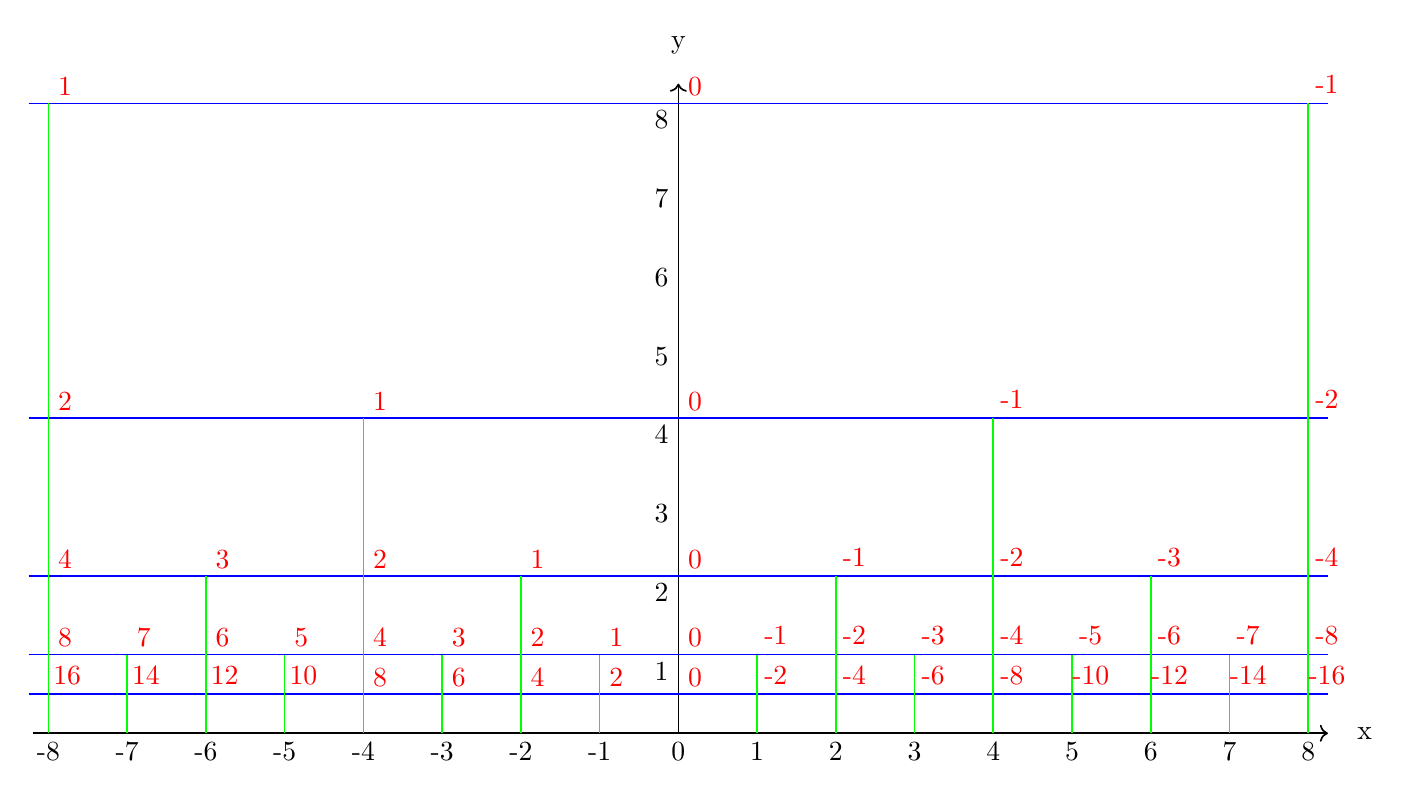
\begin{tikzpicture}
\draw [black, line width=0.6pt, ->] (0,0) to[out=90,in=270] (0,8.25);
\node [anchor=south] at (0,8.5) {y};
\draw [black, line width=0.6pt, ->] (-8.2,0) to[out=0,in=180] (8.25,0);
\node [anchor=west] at (8.5,0) {x};
\foreach \x in {-8,-7,-6,-5,-4,-3,-2,-1,0,1,2,3,4,5,6,7,8}
  \node [anchor=north] at (\x,0) {\x};
\foreach \y in {1,2,3,4,5,6,7,8}
  \node [anchor=45] at (0,\y) {\y};

\draw [blue, line width=0.6pt] (-8.25,0.5) to[out=0,in=180] (8.25,0.5);
\draw [blue, line width=0.6pt] (-8.25,1) to[out=0,in=180] (8.25,1);
\draw [blue, line width=0.6pt] (-8.25,2) to[out=0,in=180] (8.25,2);
\draw [blue, line width=0.6pt] (-8.25,4) to[out=0,in=180] (8.25,4);
\draw [blue, line width=0.6pt] (-8.25,8) to[out=0,in=180] (8.25,8);

\draw [green, line width=0.6pt] (-8,0) to[out=90,in=270] (-8,1);
\draw [green, line width=0.6pt] (-7,0) to[out=90,in=270] (-7,1);
\draw [green, line width=0.6pt] (-6,0) to[out=90,in=270] (-6,1);
\draw [green, line width=0.6pt] (-5,0) to[out=90,in=270] (-5,1);
\draw [green, line width=0.6pt] (-4,0) to[out=90,in=270] (-4,1);
\draw [green, line width=0.6pt] (-3,0) to[out=90,in=270] (-3,1);
\draw [green, line width=0.6pt] (-2,0) to[out=90,in=270] (-2,1);
\draw [green, line width=0.6pt] (-1,0) to[out=90,in=270] (-1,1);
\draw [green, line width=0.6pt] (1,0) to[out=90,in=270] (1,1);
\draw [green, line width=0.6pt] (2,0) to[out=90,in=270] (2,1);
\draw [green, line width=0.6pt] (3,0) to[out=90,in=270] (3,1);
\draw [green, line width=0.6pt] (4,0) to[out=90,in=270] (4,1);
\draw [green, line width=0.6pt] (5,0) to[out=90,in=270] (5,1);
\draw [green, line width=0.6pt] (6,0) to[out=90,in=270] (6,1);
\draw [green, line width=0.6pt] (7,0) to[out=90,in=270] (7,1);
\draw [green, line width=0.6pt] (8,0) to[out=90,in=270] (8,1);

\draw [green, line width=0.6pt] (-8,1) to[out=90,in=270] (-8,2);
\draw [green, line width=0.6pt] (-6,1) to[out=90,in=270] (-6,2);
\draw [green, line width=0.6pt] (-4,1) to[out=90,in=270] (-4,2);
\draw [green, line width=0.6pt] (-2,1) to[out=90,in=270] (-2,2);
\draw [green, line width=0.6pt] (2,1) to[out=90,in=270] (2,2);
\draw [green, line width=0.6pt] (4,1) to[out=90,in=270] (4,2);
\draw [green, line width=0.6pt] (6,1) to[out=90,in=270] (6,2);
\draw [green, line width=0.6pt] (8,1) to[out=90,in=270] (8,2);

\draw [green, line width=0.6pt] (-8,2) to[out=90,in=270] (-8,4);
\draw [green, line width=0.6pt] (-4,2) to[out=90,in=270] (-4,4);
\draw [green, line width=0.6pt] (4,2) to[out=90,in=270] (4,4);
\draw [green, line width=0.6pt] (8,2) to[out=90,in=270] (8,4);

\draw [green, line width=0.6pt] (-8,4) to[out=90,in=270] (-8,8);
\draw [green, line width=0.6pt] (8,4) to[out=90,in=270] (8,8);

\node [anchor=225, red] at (-8,0.5) {16};
\node [anchor=225, red] at (-7,0.5) {14};
\node [anchor=225, red] at (-6,0.5) {12};
\node [anchor=225, red] at (-5,0.5) {10};
\node [anchor=225, red] at (-4,0.5) {8};
\node [anchor=225, red] at (-3,0.5) {6};
\node [anchor=225, red] at (-2,0.5) {4};
\node [anchor=225, red] at (-1,0.5) {2};
\node [anchor=225, red] at (0,0.5) {0};
\node [anchor=225, red] at (1,0.5) {-2};
\node [anchor=225, red] at (2,0.5) {-4};
\node [anchor=225, red] at (3,0.5) {-6};
\node [anchor=225, red] at (4,0.5) {-8};
\node [anchor=225, red] at (5,0.5) {-10};
\node [anchor=225, red] at (6,0.5) {-12};
\node [anchor=225, red] at (7,0.5) {-14};
\node [anchor=225, red] at (8,0.5) {-16};

\node [anchor=225, red] at (-8,1) {8};
\node [anchor=225, red] at (-7,1) {7};
\node [anchor=225, red] at (-6,1) {6};
\node [anchor=225, red] at (-5,1) {5};
\node [anchor=225, red] at (-4,1) {4};
\node [anchor=225, red] at (-3,1) {3};
\node [anchor=225, red] at (-2,1) {2};
\node [anchor=225, red] at (-1,1) {1};
\node [anchor=225, red] at (0,1) {0};
\node [anchor=225, red] at (1,1) {-1};
\node [anchor=225, red] at (2,1) {-2};
\node [anchor=225, red] at (3,1) {-3};
\node [anchor=225, red] at (4,1) {-4};
\node [anchor=225, red] at (5,1) {-5};
\node [anchor=225, red] at (6,1) {-6};
\node [anchor=225, red] at (7,1) {-7};
\node [anchor=225, red] at (8,1) {-8};

\node [anchor=225, red] at (-8,2) {4};
\node [anchor=225, red] at (-6,2) {3};
\node [anchor=225, red] at (-4,2) {2};
\node [anchor=225, red] at (-2,2) {1};
\node [anchor=225, red] at (0,2) {0};
\node [anchor=225, red] at (2,2) {-1};
\node [anchor=225, red] at (4,2) {-2};
\node [anchor=225, red] at (6,2) {-3};
\node [anchor=225, red] at (8,2) {-4};

\node [anchor=225, red] at (-8,4) {2};
\node [anchor=225, red] at (-4,4) {1};
\node [anchor=225, red] at (0,4) {0};
\node [anchor=225, red] at (4,4) {-1};
\node [anchor=225, red] at (8,4) {-2};

\node [anchor=225, red] at (-8,8) {1};
\node [anchor=225, red] at (0,8) {0};
\node [anchor=225, red] at (8,8) {-1};

\end{tikzpicture}
}
\caption{加乘网格,$\lambda=\ln2$ 和 $\mu=1$}\label{fig:gridex0}
\end{figure}

考虑 $\mathcal{H}$ 上的一个标量场 $A$

\begin{equation}
   A  = - \frac{x}{y}
\end{equation}

从上面的赋值和度规,可以导出一个如图 \ref{fig:gridex0} 的加乘网格。
在加乘网格里,蓝线代表 $+ 1$ 关系,绿线代表 $\times 2$ 关系,它们是彼此垂直的线族。
蓝线之间是等间隔为长度 1 的。图里的红色数值是标量场 $A$ 的大小。
注意到蓝线和绿线各自代表的关系,我们就可以用它们来编码可线索化算术表达式了。

例如:

$$
(1 \times 2 \times 2 - 1) \times 2 - 3
$$

可以得到如图\ref{fig:pathex0}的一条路径。

\begin{figure}[ht]
\centering
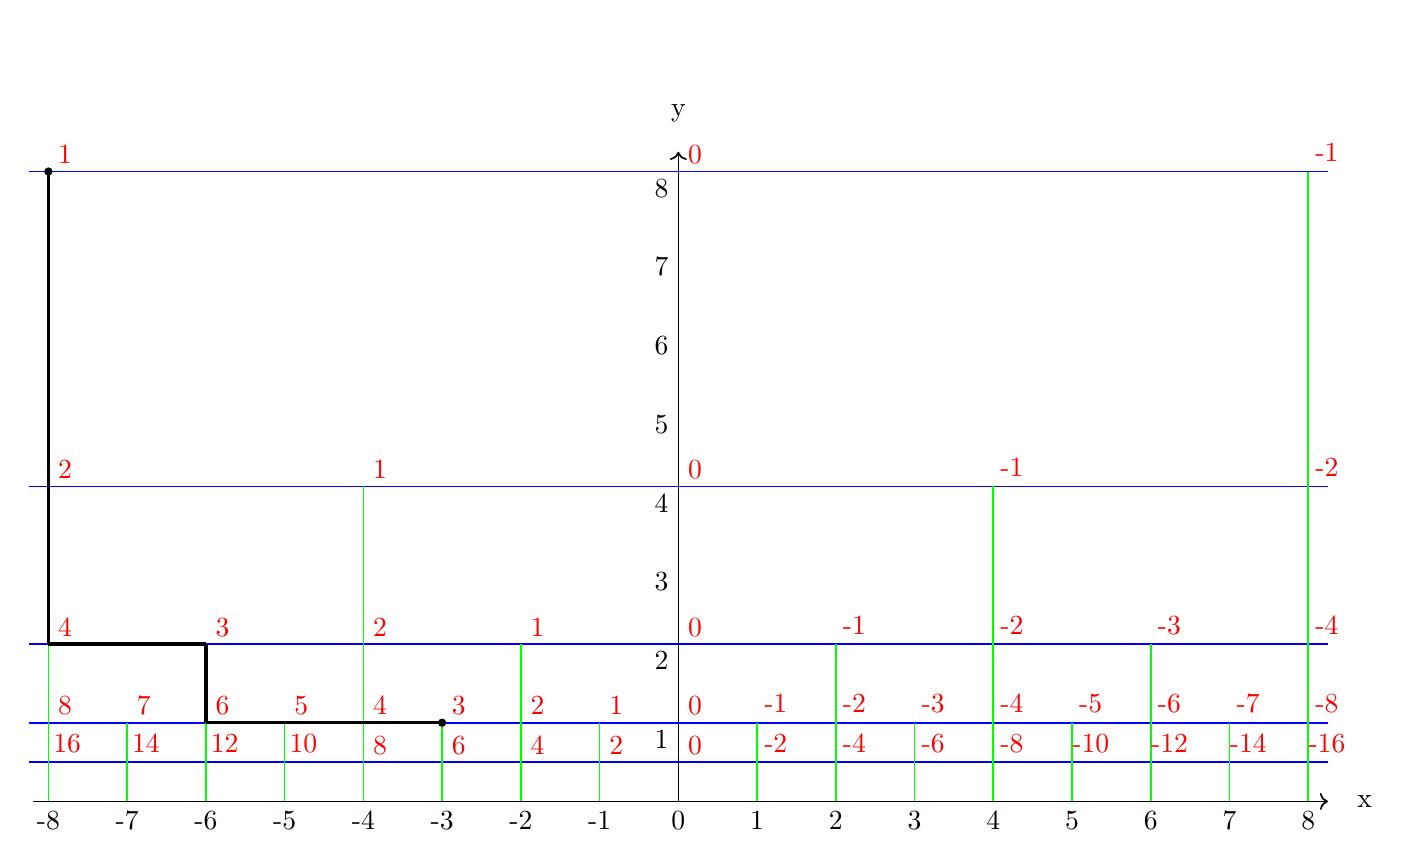
\begin{tikzpicture}
\draw [black, line width=0.6pt, ->] (0,0) to[out=90,in=270] (0,8.25);
\node [anchor=south] at (0,8.5) {y};
\draw [black, line width=0.6pt, ->] (-8.2,0) to[out=0,in=180] (8.25,0);
\node [anchor=west] at (8.5,0) {x};
\foreach \x in {-8,-7,-6,-5,-4,-3,-2,-1,0,1,2,3,4,5,6,7,8}
  \node [anchor=north] at (\x,0) {\x};
\foreach \y in {1,2,3,4,5,6,7,8}
  \node [anchor=45] at (0,\y) {\y};

\draw [blue, line width=0.6pt] (-8.25,0.5) to[out=0,in=180] (8.25,0.5);
\draw [blue, line width=0.6pt] (-8.25,1) to[out=0,in=180] (8.25,1);
\draw [blue, line width=0.6pt] (-8.25,2) to[out=0,in=180] (8.25,2);
\draw [blue, line width=0.6pt] (-8.25,4) to[out=0,in=180] (8.25,4);
\draw [blue, line width=0.6pt] (-8.25,8) to[out=0,in=180] (8.25,8);

\draw [green, line width=0.6pt] (-8,0) to[out=90,in=270] (-8,1);
\draw [green, line width=0.6pt] (-7,0) to[out=90,in=270] (-7,1);
\draw [green, line width=0.6pt] (-6,0) to[out=90,in=270] (-6,1);
\draw [green, line width=0.6pt] (-5,0) to[out=90,in=270] (-5,1);
\draw [green, line width=0.6pt] (-4,0) to[out=90,in=270] (-4,1);
\draw [green, line width=0.6pt] (-3,0) to[out=90,in=270] (-3,1);
\draw [green, line width=0.6pt] (-2,0) to[out=90,in=270] (-2,1);
\draw [green, line width=0.6pt] (-1,0) to[out=90,in=270] (-1,1);
\draw [green, line width=0.6pt] (1,0) to[out=90,in=270] (1,1);
\draw [green, line width=0.6pt] (2,0) to[out=90,in=270] (2,1);
\draw [green, line width=0.6pt] (3,0) to[out=90,in=270] (3,1);
\draw [green, line width=0.6pt] (4,0) to[out=90,in=270] (4,1);
\draw [green, line width=0.6pt] (5,0) to[out=90,in=270] (5,1);
\draw [green, line width=0.6pt] (6,0) to[out=90,in=270] (6,1);
\draw [green, line width=0.6pt] (7,0) to[out=90,in=270] (7,1);
\draw [green, line width=0.6pt] (8,0) to[out=90,in=270] (8,1);

\draw [green, line width=0.6pt] (-8,1) to[out=90,in=270] (-8,2);
\draw [green, line width=0.6pt] (-6,1) to[out=90,in=270] (-6,2);
\draw [green, line width=0.6pt] (-4,1) to[out=90,in=270] (-4,2);
\draw [green, line width=0.6pt] (-2,1) to[out=90,in=270] (-2,2);
\draw [green, line width=0.6pt] (2,1) to[out=90,in=270] (2,2);
\draw [green, line width=0.6pt] (4,1) to[out=90,in=270] (4,2);
\draw [green, line width=0.6pt] (6,1) to[out=90,in=270] (6,2);
\draw [green, line width=0.6pt] (8,1) to[out=90,in=270] (8,2);

\draw [green, line width=0.6pt] (-8,2) to[out=90,in=270] (-8,4);
\draw [green, line width=0.6pt] (-4,2) to[out=90,in=270] (-4,4);
\draw [green, line width=0.6pt] (4,2) to[out=90,in=270] (4,4);
\draw [green, line width=0.6pt] (8,2) to[out=90,in=270] (8,4);

\draw [green, line width=0.6pt] (-8,4) to[out=90,in=270] (-8,8);
\draw [green, line width=0.6pt] (8,4) to[out=90,in=270] (8,8);

\node [anchor=225, red] at (-8,0.5) {16};
\node [anchor=225, red] at (-7,0.5) {14};
\node [anchor=225, red] at (-6,0.5) {12};
\node [anchor=225, red] at (-5,0.5) {10};
\node [anchor=225, red] at (-4,0.5) {8};
\node [anchor=225, red] at (-3,0.5) {6};
\node [anchor=225, red] at (-2,0.5) {4};
\node [anchor=225, red] at (-1,0.5) {2};
\node [anchor=225, red] at (0,0.5) {0};
\node [anchor=225, red] at (1,0.5) {-2};
\node [anchor=225, red] at (2,0.5) {-4};
\node [anchor=225, red] at (3,0.5) {-6};
\node [anchor=225, red] at (4,0.5) {-8};
\node [anchor=225, red] at (5,0.5) {-10};
\node [anchor=225, red] at (6,0.5) {-12};
\node [anchor=225, red] at (7,0.5) {-14};
\node [anchor=225, red] at (8,0.5) {-16};

\node [anchor=225, red] at (-8,1) {8};
\node [anchor=225, red] at (-7,1) {7};
\node [anchor=225, red] at (-6,1) {6};
\node [anchor=225, red] at (-5,1) {5};
\node [anchor=225, red] at (-4,1) {4};
\node [anchor=225, red] at (-3,1) {3};
\node [anchor=225, red] at (-2,1) {2};
\node [anchor=225, red] at (-1,1) {1};
\node [anchor=225, red] at (0,1) {0};
\node [anchor=225, red] at (1,1) {-1};
\node [anchor=225, red] at (2,1) {-2};
\node [anchor=225, red] at (3,1) {-3};
\node [anchor=225, red] at (4,1) {-4};
\node [anchor=225, red] at (5,1) {-5};
\node [anchor=225, red] at (6,1) {-6};
\node [anchor=225, red] at (7,1) {-7};
\node [anchor=225, red] at (8,1) {-8};

\node [anchor=225, red] at (-8,2) {4};
\node [anchor=225, red] at (-6,2) {3};
\node [anchor=225, red] at (-4,2) {2};
\node [anchor=225, red] at (-2,2) {1};
\node [anchor=225, red] at (0,2) {0};
\node [anchor=225, red] at (2,2) {-1};
\node [anchor=225, red] at (4,2) {-2};
\node [anchor=225, red] at (6,2) {-3};
\node [anchor=225, red] at (8,2) {-4};

\node [anchor=225, red] at (-8,4) {2};
\node [anchor=225, red] at (-4,4) {1};
\node [anchor=225, red] at (0,4) {0};
\node [anchor=225, red] at (4,4) {-1};
\node [anchor=225, red] at (8,4) {-2};

\node [anchor=225, red] at (-8,8) {1};
\node [anchor=225, red] at (0,8) {0};
\node [anchor=225, red] at (8,8) {-1};

\node[circle,fill=black,inner sep=1pt,minimum size=3pt] (a) at (-8,8) {};
\node[circle,fill=black,inner sep=1pt,minimum size=3pt] (b) at (-3,1) {};
\draw [black, line width=1.2pt] (-8,7.7) to[out=90,in=270] (-8,2.3);
\draw [black, line width=1.2pt] (-8,2) to[out=0,in=180] (-6,2);
\draw [black, line width=1.2pt] (-6,1.95) to[out=90,in=270] (-6,1.05);
\draw [black, line width=1.2pt] (-6,1) to[out=0,in=180] (-3,1);
\end{tikzpicture}
\caption{加乘网格上的一条路径(黑色粗线)}\label{fig:pathex0}
\end{figure}

下面我们先讨论连接两个点之间的典范形式。如图 \ref{fig:pathex1} ,有如下路径和对应表达式
\begin{itemize}
    \item 黑色路径:$1 \times 8 - 5 = 3$
    \item 紫色路径:$(1 - \frac{5}{8}) \times 8 = 3$
    \item 棕色路径:$(((1 - \frac{1}{8}) \times 2 - \frac{1}{2}) \times 2 - 1) \times 2 = 3$
    \item 桔色路径:代表无限多个加乘式的累积,可以理解成一种特殊的积分形态的例子
\end{itemize}

\begin{figure}[ht]
\centering
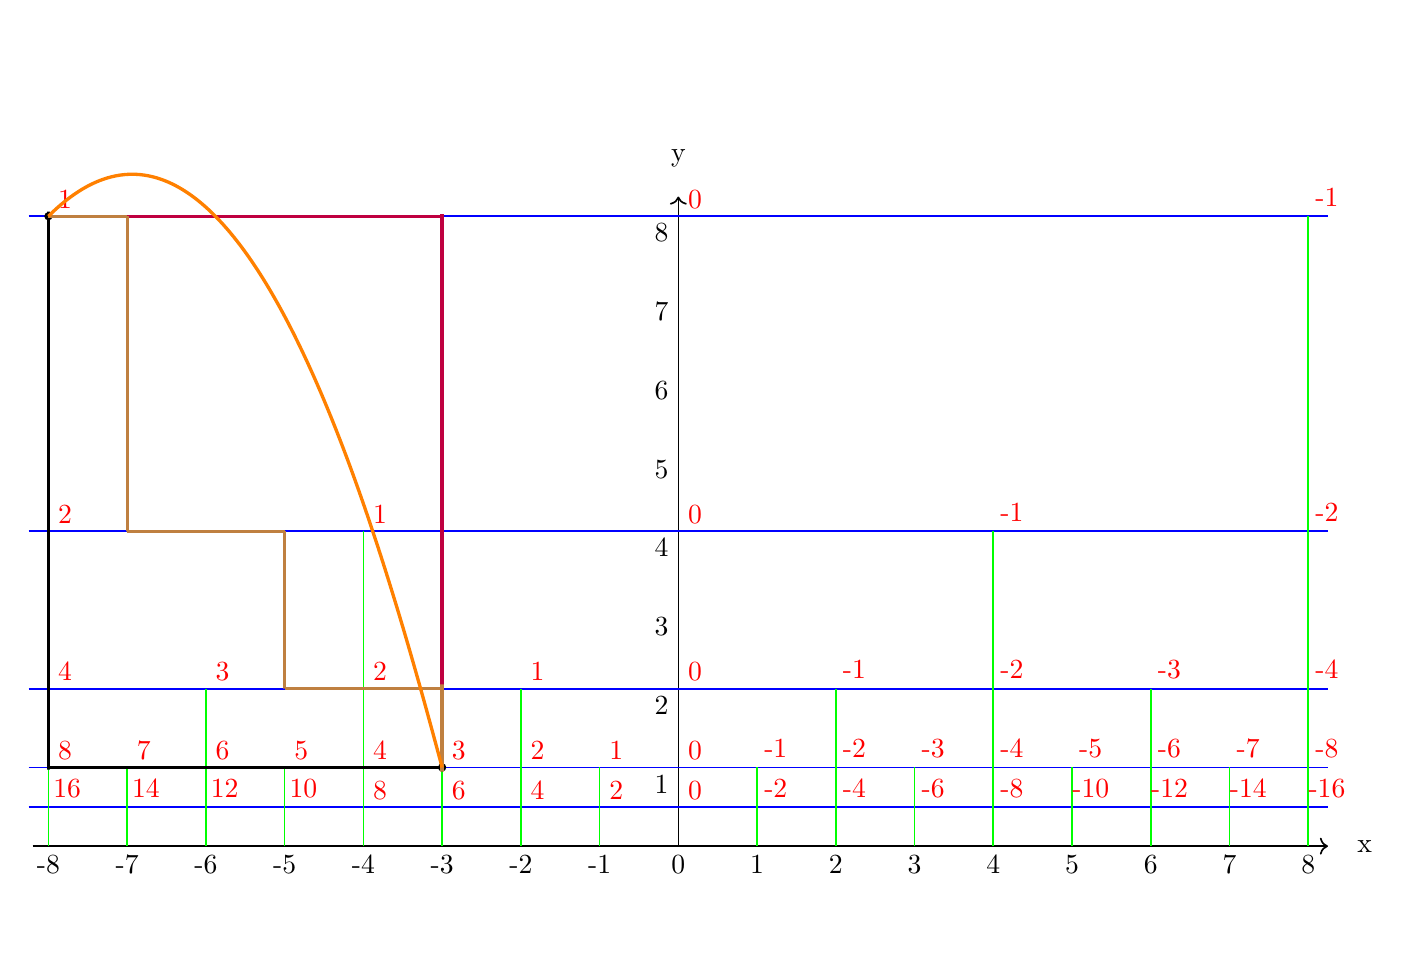
\begin{tikzpicture}
\draw [black, line width=0.6pt, ->] (0,0) to[out=90,in=270] (0,8.25);
\node [anchor=south] at (0,8.5) {y};
\draw [black, line width=0.6pt, ->] (-8.2,0) to[out=0,in=180] (8.25,0);
\node [anchor=west] at (8.5,0) {x};
\foreach \x in {-8,-7,-6,-5,-4,-3,-2,-1,0,1,2,3,4,5,6,7,8}
  \node [anchor=north] at (\x,0) {\x};
\foreach \y in {1,2,3,4,5,6,7,8}
  \node [anchor=45] at (0,\y) {\y};

\draw [blue, line width=0.6pt] (-8.25,0.5) to[out=0,in=180] (8.25,0.5);
\draw [blue, line width=0.6pt] (-8.25,1) to[out=0,in=180] (8.25,1);
\draw [blue, line width=0.6pt] (-8.25,2) to[out=0,in=180] (8.25,2);
\draw [blue, line width=0.6pt] (-8.25,4) to[out=0,in=180] (8.25,4);
\draw [blue, line width=0.6pt] (-8.25,8) to[out=0,in=180] (8.25,8);

\draw [green, line width=0.6pt] (-8,0) to[out=90,in=270] (-8,1);
\draw [green, line width=0.6pt] (-7,0) to[out=90,in=270] (-7,1);
\draw [green, line width=0.6pt] (-6,0) to[out=90,in=270] (-6,1);
\draw [green, line width=0.6pt] (-5,0) to[out=90,in=270] (-5,1);
\draw [green, line width=0.6pt] (-4,0) to[out=90,in=270] (-4,1);
\draw [green, line width=0.6pt] (-3,0) to[out=90,in=270] (-3,1);
\draw [green, line width=0.6pt] (-2,0) to[out=90,in=270] (-2,1);
\draw [green, line width=0.6pt] (-1,0) to[out=90,in=270] (-1,1);
\draw [green, line width=0.6pt] (1,0) to[out=90,in=270] (1,1);
\draw [green, line width=0.6pt] (2,0) to[out=90,in=270] (2,1);
\draw [green, line width=0.6pt] (3,0) to[out=90,in=270] (3,1);
\draw [green, line width=0.6pt] (4,0) to[out=90,in=270] (4,1);
\draw [green, line width=0.6pt] (5,0) to[out=90,in=270] (5,1);
\draw [green, line width=0.6pt] (6,0) to[out=90,in=270] (6,1);
\draw [green, line width=0.6pt] (7,0) to[out=90,in=270] (7,1);
\draw [green, line width=0.6pt] (8,0) to[out=90,in=270] (8,1);

\draw [green, line width=0.6pt] (-8,1) to[out=90,in=270] (-8,2);
\draw [green, line width=0.6pt] (-6,1) to[out=90,in=270] (-6,2);
\draw [green, line width=0.6pt] (-4,1) to[out=90,in=270] (-4,2);
\draw [green, line width=0.6pt] (-2,1) to[out=90,in=270] (-2,2);
\draw [green, line width=0.6pt] (2,1) to[out=90,in=270] (2,2);
\draw [green, line width=0.6pt] (4,1) to[out=90,in=270] (4,2);
\draw [green, line width=0.6pt] (6,1) to[out=90,in=270] (6,2);
\draw [green, line width=0.6pt] (8,1) to[out=90,in=270] (8,2);

\draw [green, line width=0.6pt] (-8,2) to[out=90,in=270] (-8,4);
\draw [green, line width=0.6pt] (-4,2) to[out=90,in=270] (-4,4);
\draw [green, line width=0.6pt] (4,2) to[out=90,in=270] (4,4);
\draw [green, line width=0.6pt] (8,2) to[out=90,in=270] (8,4);

\draw [green, line width=0.6pt] (-8,4) to[out=90,in=270] (-8,8);
\draw [green, line width=0.6pt] (8,4) to[out=90,in=270] (8,8);

\node [anchor=225, red] at (-8,0.5) {16};
\node [anchor=225, red] at (-7,0.5) {14};
\node [anchor=225, red] at (-6,0.5) {12};
\node [anchor=225, red] at (-5,0.5) {10};
\node [anchor=225, red] at (-4,0.5) {8};
\node [anchor=225, red] at (-3,0.5) {6};
\node [anchor=225, red] at (-2,0.5) {4};
\node [anchor=225, red] at (-1,0.5) {2};
\node [anchor=225, red] at (0,0.5) {0};
\node [anchor=225, red] at (1,0.5) {-2};
\node [anchor=225, red] at (2,0.5) {-4};
\node [anchor=225, red] at (3,0.5) {-6};
\node [anchor=225, red] at (4,0.5) {-8};
\node [anchor=225, red] at (5,0.5) {-10};
\node [anchor=225, red] at (6,0.5) {-12};
\node [anchor=225, red] at (7,0.5) {-14};
\node [anchor=225, red] at (8,0.5) {-16};

\node [anchor=225, red] at (-8,1) {8};
\node [anchor=225, red] at (-7,1) {7};
\node [anchor=225, red] at (-6,1) {6};
\node [anchor=225, red] at (-5,1) {5};
\node [anchor=225, red] at (-4,1) {4};
\node [anchor=225, red] at (-3,1) {3};
\node [anchor=225, red] at (-2,1) {2};
\node [anchor=225, red] at (-1,1) {1};
\node [anchor=225, red] at (0,1) {0};
\node [anchor=225, red] at (1,1) {-1};
\node [anchor=225, red] at (2,1) {-2};
\node [anchor=225, red] at (3,1) {-3};
\node [anchor=225, red] at (4,1) {-4};
\node [anchor=225, red] at (5,1) {-5};
\node [anchor=225, red] at (6,1) {-6};
\node [anchor=225, red] at (7,1) {-7};
\node [anchor=225, red] at (8,1) {-8};

\node [anchor=225, red] at (-8,2) {4};
\node [anchor=225, red] at (-6,2) {3};
\node [anchor=225, red] at (-4,2) {2};
\node [anchor=225, red] at (-2,2) {1};
\node [anchor=225, red] at (0,2) {0};
\node [anchor=225, red] at (2,2) {-1};
\node [anchor=225, red] at (4,2) {-2};
\node [anchor=225, red] at (6,2) {-3};
\node [anchor=225, red] at (8,2) {-4};

\node [anchor=225, red] at (-8,4) {2};
\node [anchor=225, red] at (-4,4) {1};
\node [anchor=225, red] at (0,4) {0};
\node [anchor=225, red] at (4,4) {-1};
\node [anchor=225, red] at (8,4) {-2};

\node [anchor=225, red] at (-8,8) {1};
\node [anchor=225, red] at (0,8) {0};
\node [anchor=225, red] at (8,8) {-1};

\node[circle,fill=black,inner sep=1pt,minimum size=3pt] (a) at (-8,8) {};
\node[circle,fill=black,inner sep=1pt,minimum size=3pt] (b) at (-3,1) {};

\draw [black, line width=1.2pt] (-8,7.7) to[out=90,in=270] (-8,1.33);
\draw [black, line width=1.2pt] (-8,1) to[out=0,in=180] (-3,1);

\draw [purple, line width=1.2pt] (-8,8) to[out=0,in=180] (-3,8);
\draw [purple, line width=1.2pt] (-3,7.67) to[out=90,in=270] (-3,1.33);

\draw [brown, line width=1.2pt] (-8,8) to[out=0,in=180] (-7,8);
\draw [brown, line width=1.2pt] (-7,7.8) to[out=90,in=270] (-7,4.2);
\draw [brown, line width=1.2pt] (-7,4) to[out=0,in=180] (-5,4);
\draw [brown, line width=1.2pt] (-5,3.9) to[out=90,in=270] (-5,2.1);
\draw [brown, line width=1.2pt] (-5,2) to[out=0,in=180] (-3,2);
\draw [brown, line width=1.2pt] (-3,2) to[out=90,in=270] (-3,1);

\draw [orange, line width=1.2pt] (-8,8) to[out=45,in=105] (-3,1);

\end{tikzpicture}
\caption{连接两点的多条路径}\label{fig:pathex1}
\end{figure}

可以理解,在乘法分配律作用下,把一些项合并与拆解,上述几个表达式可以互相转化。

从棕到黑的路径转化
\begin{align}
3 & = (((1 - \frac{1}{8}) \times 2 - \frac{1}{2}) \times 2 - 1) \times 2 \\
& = 1 \times 8 -  \frac{1}{8} \times 8 - \frac{1}{2} \times 4 - 1 \times 2 \\
& = 1 \times 8 - 5
\end{align}

从棕到紫的路径转化
\begin{align}
3 & = (((1 - \frac{1}{8}) \times 2 - \frac{1}{2}) \times 2 - 1) \times 2 \\
& = (1 - \frac{1}{8}) \times 8 - \frac{1}{2} \times 4 -  1 \times 2 \\
& = (1 - \frac{1}{8}) \times 8 - \frac{1}{4} \times 8 -  \frac{1}{4} \times 8 \\
& = (1 - \frac{1}{8} - \frac{1}{4} - \frac{1}{4}) \times 8 \\
& = (1 - \frac{5}{8}) \times 8
\end{align}

我们可规定黑、紫路径是一对典范路径,所有连接如上图的赋值 $1$ 和 $3$ 之间的路径,
都可以转换到这对典范路径上。有了连接两点的典范路径,任意给定空间里的一个原点$O$,对空间里的任一点$P$,
连接$O$、$P$的典范路径就给出了相对于$O$点的整个空间的典范形式。

\subsection{流方程的引入}

下面我们引入流方程,去刻画一个无穷小范围内的表达式生成。假设加法生成元是 $\mu$,乘法生成元是 $e^\lambda$, 我们可以建立方程

\begin{equation}
    a_{\delta} = (a_0 + \mu \epsilon \cos \theta)e^{\lambda \epsilon \sin \theta}
\end{equation}

或者

\begin{equation}
    a_{\delta} = a_0 e^{\lambda \epsilon \sin \theta} + \mu \epsilon \cos \theta
\end{equation}

二者可化简为

\begin{equation}
    a_{\delta} = a_0 + \epsilon (a_0 \lambda \sin \theta + \mu \cos \theta)
\end{equation}

于是

\begin{equation}
    \frac{1}{\delta} (a_{\delta} - a_0) = \frac{\epsilon}{\delta} (\mu \cos \theta + x_0 \lambda \sin \theta)
\end{equation}

当 $\delta$ 和 $\epsilon$ 同时趋于零,就得到了 $da / dt$,即

\begin{equation}
    \frac{da}{dt} = u (\mu \cos \theta + a \lambda \sin \theta)
\end{equation}

也可改写为其他形式

\begin{equation}
    \frac{da}{ds} = \mu \cos \theta + a \lambda \sin \theta\label{eq:flow}
\end{equation}

可证上节的例子满足流方程,在附件一里可以找到证明。

\subsection{梯度-等值线坐标系}

易导出局部坐标系下的等值线方程

\begin{equation}
    \mu \cos \theta_c + a \lambda \sin \theta_c = 0
\end{equation}

故有

\begin{equation}
    \theta_c = - \arctan \frac{\mu}{a \lambda}
\end{equation}

等值线和梯度两者彼此垂直

\begin{equation}
    \theta_g = \pm \frac{\pi}{2} - \arctan \frac{\mu}{a \lambda}
\end{equation}

故沿 $\theta_g$ 我们有

\begin{equation}
    \frac{da}{ds} = \mu \cos (\pm \frac{\pi}{2} - \arctan \frac{\mu}{a \lambda}) + a \lambda \sin (\pm \frac{\pi}{2} - \arctan \frac{\mu}{a \lambda})
\end{equation}

\begin{equation}
    \frac{da}{ds} = \pm \sqrt{\mu^2 + \lambda^2 a^2}\label{eq:grad}
\end{equation}

方程 \eqref{eq:grad} 可解,得到了沿梯度流线 $a$ 和 $s$ 的关系:

\begin{equation}
    \pm \tanh(\lambda s + c) = \frac{\lambda a}{\sqrt{\mu^2 + \lambda^2 a^2}}
\end{equation}

如约定 $\mu > 0$,可进一步变形:

\begin{equation}
  a = \pm \frac{\mu}{\lambda} \sinh(c \pm \lambda s)\label{eq:gradevo}
\end{equation}

在梯度方向的基础上按右手螺旋引入转角 $\phi$,建立梯度-等值线为参照的局部极坐标系,则沿角 $\phi$ 移动时 $a$ 的增长率为

\begin{equation}
    \frac{da}{ds} = \mu \cos (\frac{\pi}{2} - \arctan \frac{\mu}{a \lambda} + \phi) + a \lambda \sin (\frac{\pi}{2} - \arctan \frac{\mu}{a \lambda} + \phi)
    \label{eq:fourfold}
\end{equation}

化简得

\begin{equation}
    \frac{da}{ds} = \sqrt {\mu^2 + a^2 \lambda^2} \cos \phi\label{eq:contourgradient}
\end{equation}

此即梯度-等值线坐标系下的流方程。

在这个坐标系下,加线和乘线分别为:

\begin{equation}
    \phi = \arccos \frac{\mu}{\sqrt {\mu^2 + a^2 \lambda^2}} \label{eq:additionalline}
\end{equation}

\begin{equation}
    \phi = \arccos \frac{a \lambda}{\sqrt {\mu^2 + a^2 \lambda^2}}\label {eq:mulitiplcativeline}
\end{equation}

通过分析这里的公式,最后我们还能得到一个赋值的几何意义。在截面曲率为$\kappa$ 的双曲平面上,半径为 $r$ 的圆面积由下式给出

\begin{equation}
2 \pi \int_0^r \left(\frac{\sinh(\sqrt{\kappa} t)}{\sqrt{\kappa}}\right) \, \mathrm{d}t\label{eq:circlearea}
\end{equation}

注意到 式\ref{eq:gradevo}和式\ref{eq:circlearea}在$c=0$时的相似性,就会把我们导向下一节几何式的分析。

\subsection{Laplace 算子的特征向量?}

为什么给到的例子里赋值是 Laplace 算子的特征向量?这会是非常有趣的几何问题。我们下面给出一个可能的工作思路。
让我们考虑一般的黎曼曲面和它上面的可能赋值。

赋值的几何意义是什么?通过一些计算,不难发现,我们在某处敲动一下施加一个小扰动,并令其匀速传播,那么传播波纹的外沿作为一个闭曲线,
它围成的面积和这个扰动生成的赋值有正比关系。

从这个角度就不难理解,赋值一定是 Laplace 算子的某些特定的特征值。因为只有这样,
传播波纹的外沿的闭曲线才能按照恰当的周期来接触,形成驻波,使得整个流形上有一个一致的赋值。所以,赋值同敲这个流形发出声音的频率有关系。

而且直观上也会发现,对于一般的黎曼曲面,传播波纹的外沿围成的面积,它的增长规律会背离球面上的同类面积的增长规律,这个背离同谱有关系,可以导出面积不等式。

如果我们考虑传播波纹的外沿的触碰,会发现触碰存在一个第几次触碰的次数。对一个给定的次数,我们把首先出现的若干个该次数的点在流形上标出来,
这些点的分布和曲率关系,它控制了流形背离球面的程度和单值化时复叠的方式。如果我们把视角从梯度等值线换为加乘的观点,就会强烈怀疑这些点和加乘网格的组织紧密联系。

以上的描述,只是适合一个零点的情况。对于连续零线,我们必须讨论零线的生成、零线是否在黎曼曲面上封闭、零线上每个点扰动出去后是否能形成驻波、
零线与黎曼面的内在对称性……

针对上面的讨论,可能会有多种可能的情况:

(一):我们沿着零线移动一个零点,每个零点都能产生同一个频率的驻波,这样把这些震动适当线性叠加,就得到了一个合适的赋值。

(二):零线只有离散个零点具有特定的频率,其他的零点由于对称性,会彼此抵消掉,反而最终剩下那些特定离散零点的震动。

……

\subsection{第二个例子的构造大意}

式\ref{eq:gradevo} 给到了 $a$ 和 $s$ 的关系,启发我们用火烧法去研究与零线等距的超圆族。

\begin{figure}[ht]
\centering
\begin{tikzpicture}
    \tkzDefPoint(0,0){O}
    \tkzDefPoint(-4,0){O1}
    \tkzDefPoint(4,0){O2}
    \tkzDefPoint(0,-4){V1}
    \tkzDefPoint(0,4){V2}
    \tkzDefPoint(0,-5){K2}
    \tkzDefPoint(0,1.44){X}

    \tkzDefCircle[apollonius,K=2](O1,O2) \tkzGetPoint{K1} \tkzGetPoints{A}{B} \tkzGetLength{rAB}
    \tkzInterCC(O,O2)(K1,A) \tkzGetPoints{C}{D}

    \tkzDrawCircle[color=red,fill=red](O,O1)
    \tkzDrawArc[R with nodes,color=green](K1,\rAB)(C,D)
    \tkzDrawArc[R with nodes,color=blue](K2,183 pt)(O2,O1)

    \tkzDefMidPoint(O,V2) \tkzGetPoint{M}
    \tkzInterLC(M,O2)(K1,A) \tkzGetPoints{N}{L}
    \tkzDrawArc[R with nodes,color=green](K1, \rAB)(N,A)

    \tkzDrawSegment[color=blue](O1,O2)
    \tkzDrawSegment[color=green](V1,V2)
    \tkzDrawCircle[R,fill=black](N,0.05 pt)
    \tkzDrawCircle[R,fill=black](A,0.05 pt)
    \tkzDrawCircle[R,fill=black](O,0.05 pt)
    \tkzDrawCircle[R,fill=black](X,0.05 pt)

    \tkzLabelPoint[below right](A){$P$}
    \tkzLabelPoint[above right](N){$Q$}
    \tkzLabelPoint[below left](O1){$\Omega_r$}
    \tkzLabelPoint[below right](O2){$\Omega_l$}
    \tkzLabelPoint[below](V1){$\Omega_b$}
    \tkzLabelPoint[above](V2){$\Omega_a$}
    \tkzLabelPoint[below left](O){$O$}
    \tkzLabelPoint[above left](X){$R$}
    \tkzLabelLine[blue,left](A,N){$s$}
    \tkzLabelLine[blue,left](O,X){$s$}
\end{tikzpicture}
\caption{沿着超圆的对称性}\label{fig:appolo}
\end{figure}

如图\ref{fig:appolo},我们从零线 $\Omega_r O \Omega_l$ 开始燃烧,超圆$\Omega_r R \Omega_l$ 各处距离零线都为 $s$ 。
所以,当我们沿超圆从 $R$ 移动到 $Q$ ,同时零线上的 $O$ 移动到了 $P$,在这个过程中,距离 $s$ 保持不变,反映了一种平移运动中的对称性。

如图\ref{fig:merged},当我们把这种对称性和四阶无限边形铺嵌结合在一起观察的时候,
我们会发现,平移对称性适当离散化后,可以保持四阶无限边形铺嵌不变。

\begin{figure}[ht]
\centering

\begin{tikzpicture}
\begin{scope}[line width=0.3pt]
    \draw (0, 0) node[inner sep=0] {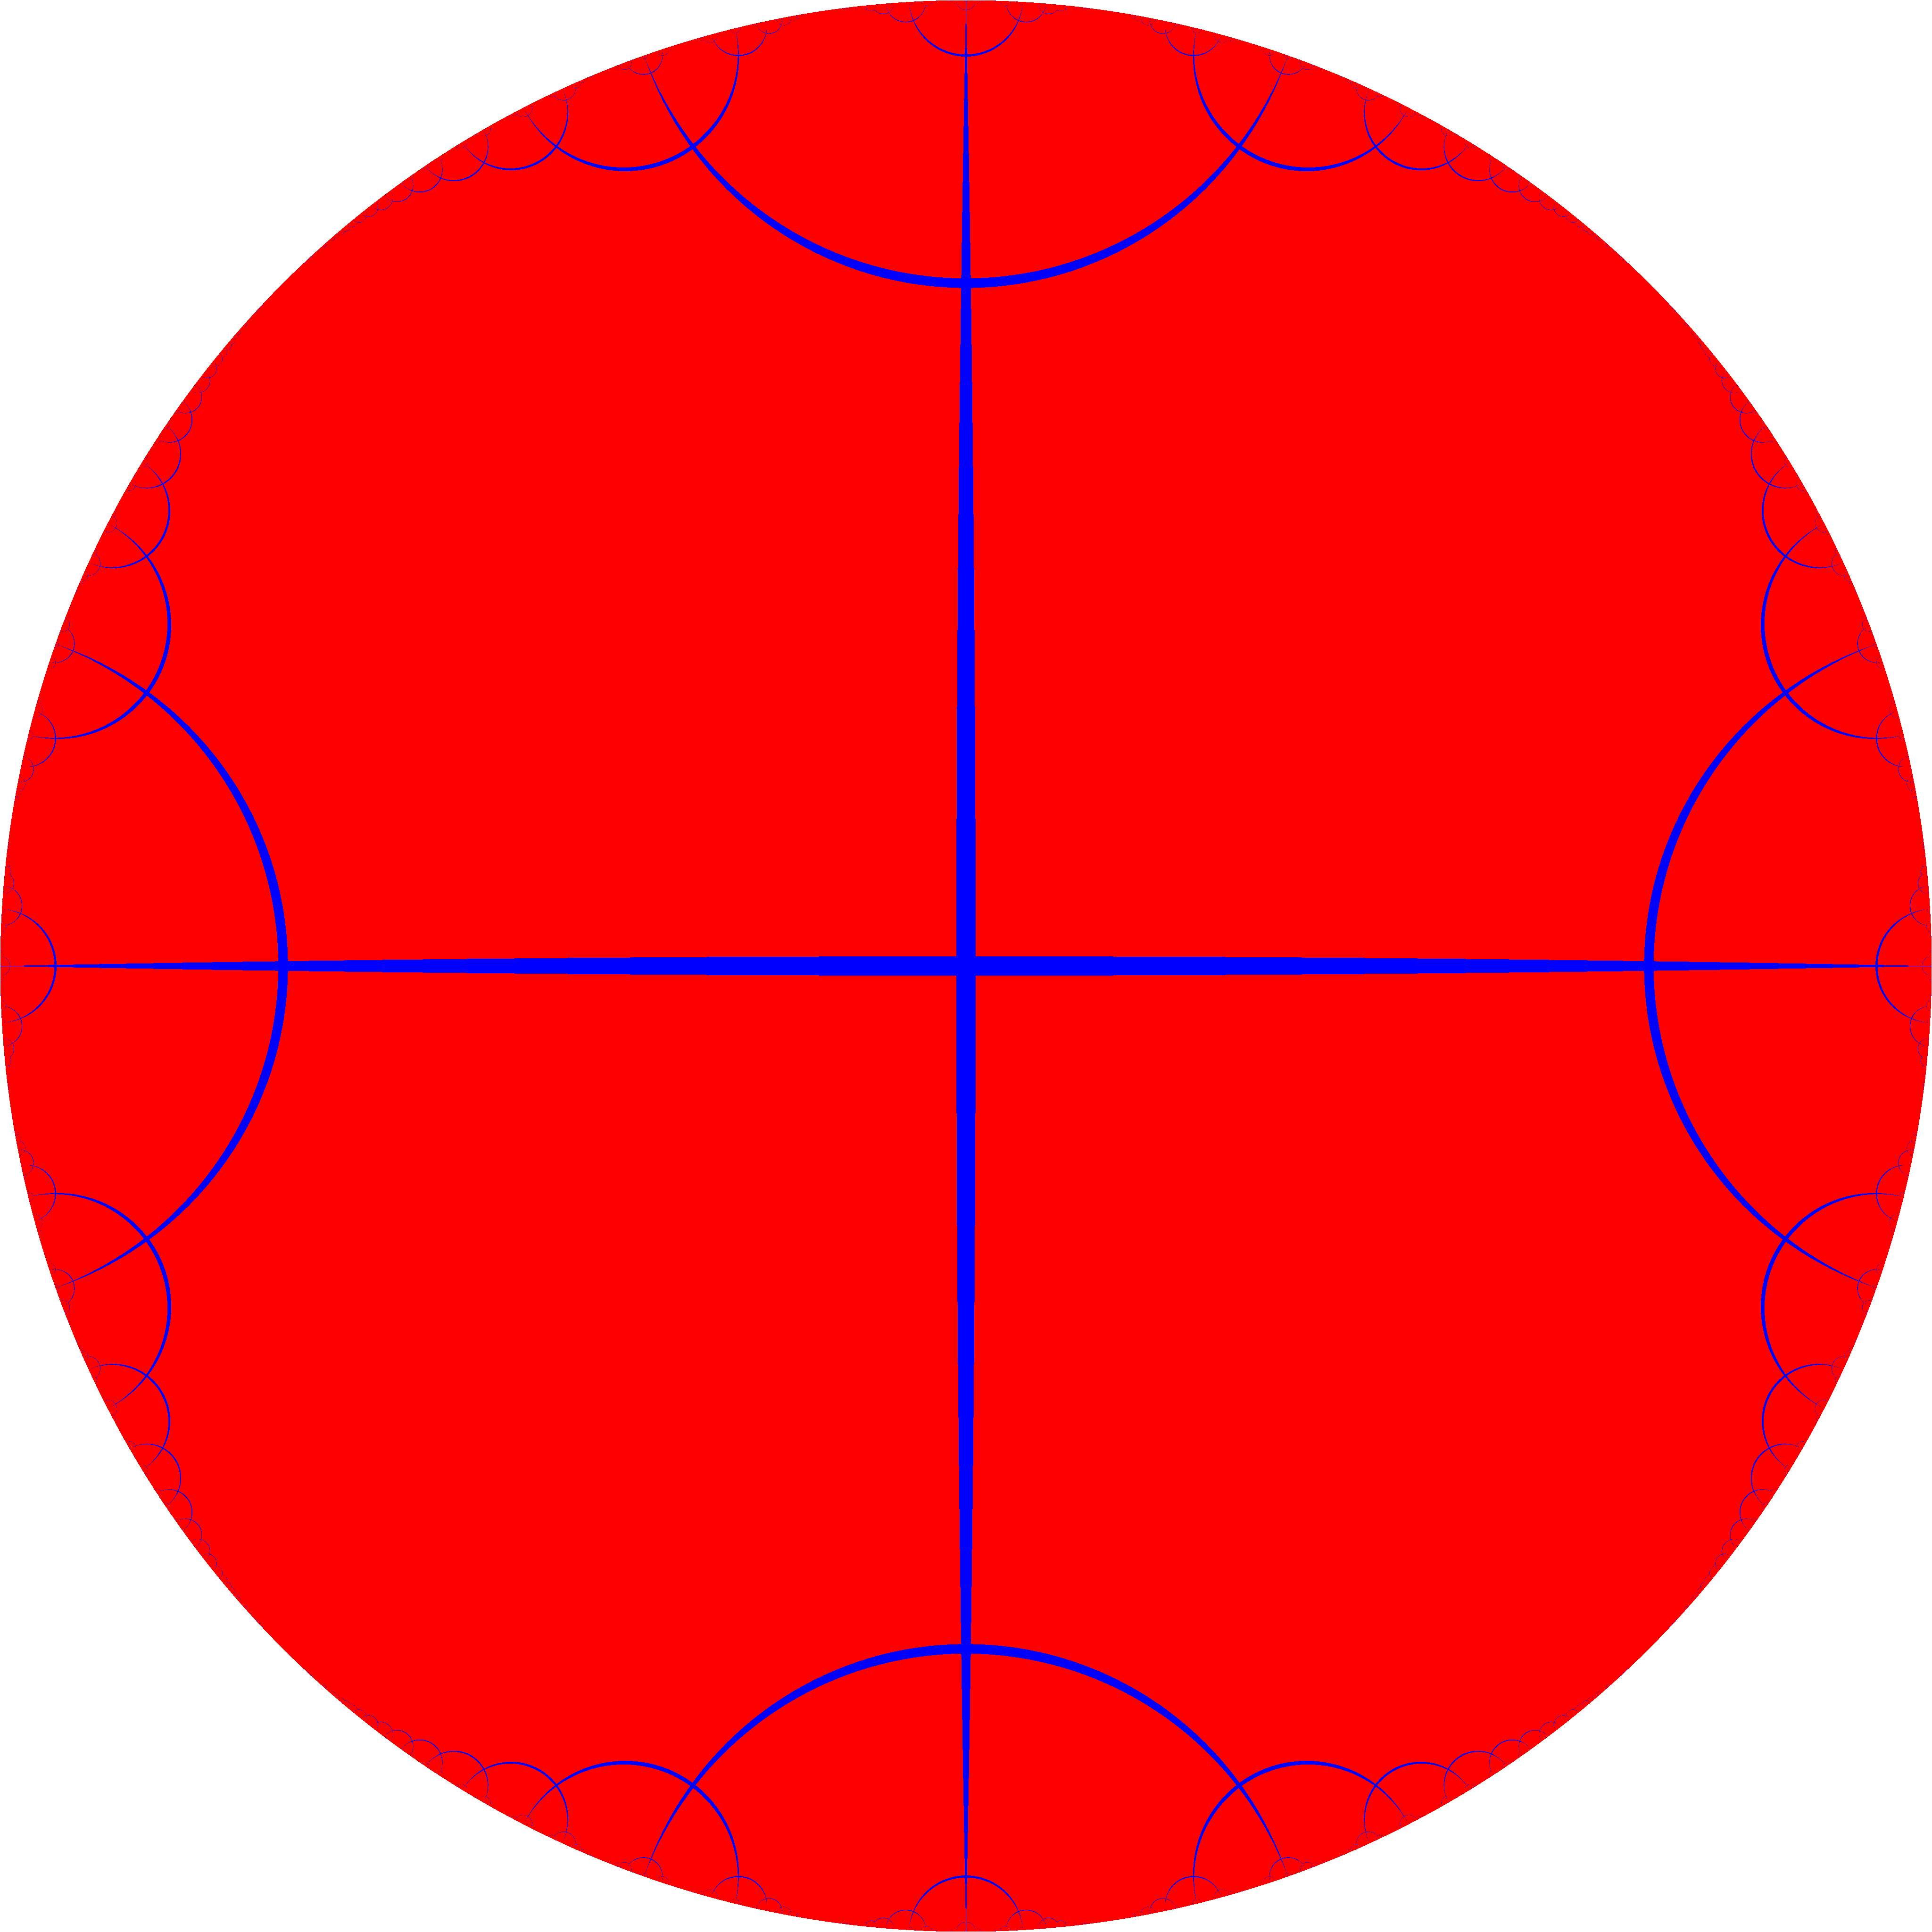
\includegraphics[width=3.142in]{images/t4097.png}};
    \tkzDefPoint(0,0){O}
    \tkzDefPoint(-4,0){O1}
    \tkzDefPoint(4,0){O2}
    \tkzDefPoint(0,-4){V1}
    \tkzDefPoint(0,4){V2}
    \tkzDefPoint(-5, 0){K2}

    \tkzDefCircle[apollonius,K=2.415](V1,V2) \tkzGetPoint{K1} \tkzGetPoints{A}{B} \tkzGetLength{rAp}
    \tkzInterCC(O,V2)(K1,A) \tkzGetPoints{C}{D}
    \tkzInterCC(K2,V2)(K1,A) \tkzGetPoints{L}{N}

    \tkzDrawCircle[color=black](O,V1)
    \tkzDrawArc[R with nodes,color=gray](K1,\rAp)(C,D)
    \tkzDrawArc[R with nodes,color=yellow](K2,1.8)(V1,V2)

    \tkzDrawSegment[color=blue](O1,O2)
    \tkzDrawSegment[color=blue](V1,V2)
    \tkzDrawCircle[R,fill=black](N,0.02)

    \tkzLabelPoint[below](V1){$\Omega_{s}$}
    \tkzLabelPoint[above](V2){$\Omega_{n}$}
    \tkzLabelLine[blue,above](A,N){$s$}

    \tkzDefPoint(2.82,0){P}
    \tkzDefPoint(3.36,1.13){Q}
    \tkzDefPoint(4,0){R}
    \tkzDefPoint(3.773,1.32){S}
    \tkzDrawCircle[R,fill=black](O,0.02)
    \tkzDrawCircle[R,fill=black](P,0.02)
    \tkzDrawCircle[R,fill=black](Q,0.02)
    \tkzDrawCircle[R,fill=black](R,0.02)
    \tkzDrawCircle[R,fill=black](S,0.02)
    \tkzLabelPoint[below left](O){$O$}
    \tkzLabelPoint[below left](P){$P$}
    \tkzLabelPoint[left](Q){$Q$}
    \tkzLabelPoint[right](R){$\Omega_{1}$}
    \tkzLabelPoint[right](S){$\Omega_{2}$}

\end{scope}
\end{tikzpicture}
\caption{四阶无限边形铺嵌里的对称性}\label{fig:merged}
\end{figure}

另一方面,当火线离开零线推进的时候,我们可以观察到,火线的梯度方向和四阶无限边形存在如下的搭配关系:

\begin{itemize}
    \item 火线沿 $O\Omega_{1}$ 向前传播,梯度方向始终和 $O\Omega_{1}$ 一致。
    \item 火线到达 $P$ 点,$PQ$ 上每点的切线都与火线到达时的梯度,它们的夹角会均匀地从 $\frac{\pi}{2}$ 变化到 $0$。
    \item 于是进一步,火线沿 $Q\Omega_{2}$ 向前传播,梯度方向始终和 $Q\Omega_{2}$ 一致。
    \item 上述情况反复出现……
\end{itemize}

这些直观的观察是在讨论四阶无限边形铺嵌的某种对称性。围绕这个对称性,结合公式 \ref{eq:fourfold} ,
就可以对无限边形染色,其中的每种颜色代表前述公式里一种符号的选择。

\subsection{四阶无限边形铺嵌里的问题}

第二个例子目前还没能严格化,主要障碍是四阶无限边形铺嵌的详细构造还没有严格给出。但我们通过数值计算已经得到一些有用的思路。

\begin{figure}[ht]
    \centering
    \begin{tikzpicture}
        \begin{scope}[line width=0.3pt]
            \draw (0, 0) node[inner sep=0] {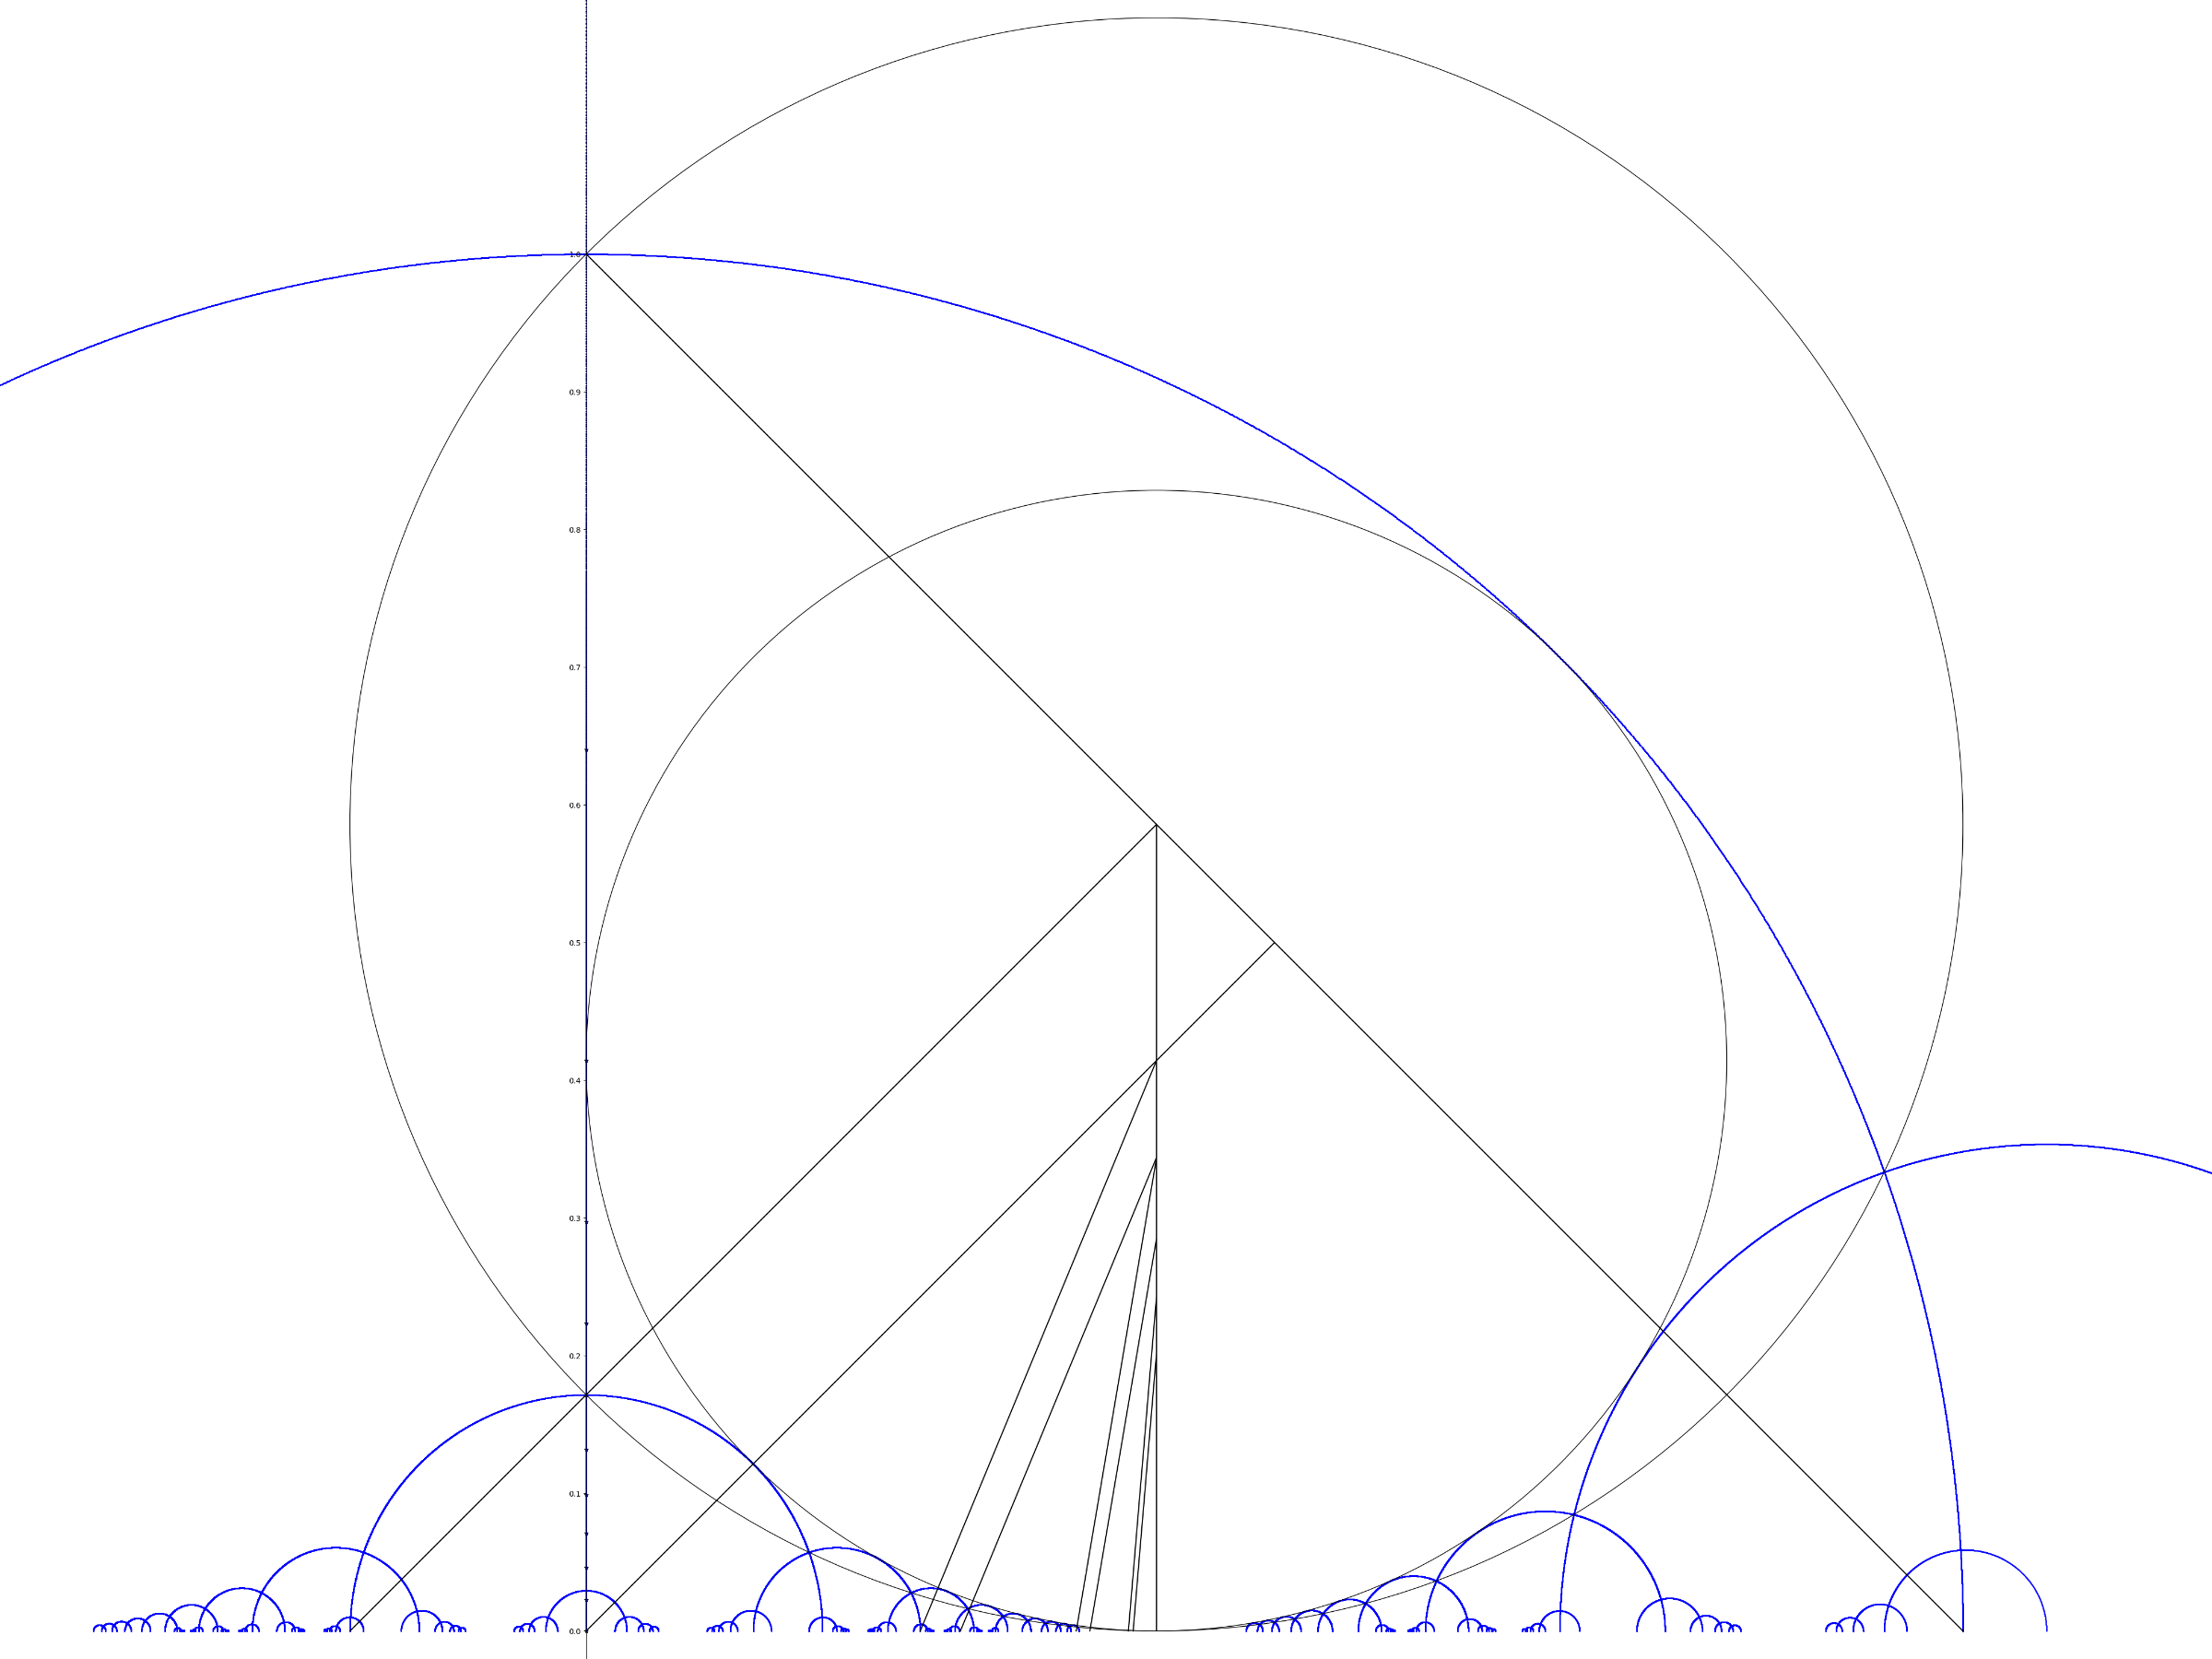
\includegraphics[width=6.284in]{images/apeirogon.png}};
        \end{scope}
    \end{tikzpicture}
    \caption{四阶无限边形铺嵌}\label{fig:apeirogon}
\end{figure}

我们发现用上半平面模型计算四阶无限边形铺嵌的构造细节是最方便的,不涉及超越函数。它被化归为一个 Apollonian gasket 的构造。
一个四阶无限边形臂都有共同的切圆和接圆。我们数值求出了切圆和接圆的坐标,并规范到严格的表达式。
作为副产品,这个构造过程可以导出一个类似 Calkin–Wilf 生成树一样的 $\mathbb{Q}[\sqrt{2}]$ 的生成树。
但仍然需要去严格证明这个从数值模拟得到的构造成立。

为了证明四阶无限边形铺嵌的构造成立,我们需证明上图中存在一个趋于零的点列$p_i$,同时伴随一个二等分角的序列。
理论上可以通过数学归纳法,在初等几何下证明该命题,但计算过于繁复,目前还没有走通。

数值计算的结果可以参看图 \ref{fig:apeirogon},图中可以观察到二等分角的序列,以及y坐标上的等比数列。
这里面会观察到二等分角的射线同切圆、接圆的关系并不简单,会有一些切圆、接圆不被射线接触到,于是就形成了一连串空档。
这些空档里的圆的个数的呈现规律,会极大的影响这个问题的难度。如果空档里的圆的个数有递归公式,就意味着四阶无限边形铺嵌是比较平凡的构造。
但如果空档里的圆的个数呈现非平凡的规律,就意味着这个问题非常之难。目前,数值实验的迭代深度还不够,还无法就上面这个空档的规律给出意见。

\subsection{复化与对偶的想法}

经过一段时间的思考和探索,和朋友\footnote{受教于蒋文峰、陈越老师的指导}的讨论与指导,产生了一些想法,还没有经受足够多例子的验算与严格证明的支持。
我犹豫再三决定还是写上,虽然可能还有错误,但代表了一种思考方向。

在算法的领域,我们常常能够发现算法的效率和数据结构之间存在一定的对易关系。数据结构精巧复杂,算法就可能会快一些;反之,数据结构朴素直白,算法可能就会慢一些。
在我们这里,算术表达式的典范形态相当于一种表达式的组织方式,而几何流相当于算法的执行。Laplace 算子出现在这里,让我们不能不想到大数乘法的快速算法里
有 FFT 的出现,而 FFT 本身就是来自调和分析。这给到我们一个暗示,有没有可能典范形态对应空间复杂度,几何流对应时间复杂度?于是,恰当的典范形态就是一张
缓缓张开的极小曲面?

我们已经观察到赋值是 Laplace 算子的某些特征向量,同时共形变换保持流方程不变,但特征值不是共形不变量,特征值的模平方是共形不变量。
这就引导我们去想把问题适当的复化,同时还要保持原始问题里的信息。梯度-等值线坐标给出以后,在一定边界条件下,我们或许可以研究把梯度和等值线的地位互易,
这样总共得到两个函数,然后对它们复化。

这个想法的基本动机是这样:特征值模平方不变是一个圆,不妨称为特征圆。有没有这样的可能?
赋值 $A$ 有等值线和梯度线,我们交换等值线和梯度线的地位,并在适当的边界条件下,得到 $A$ 的共轭 $B$。
我们对 $A$、$B$ 都施加同样的共形变换并加以观察。在某些情况下,$A$ 会变成一个调和函数 $f$,类似, $B$ 在某些情况下也会变为一个调和函数 $g$。
当我们同时观察 $A$、$B$,有种很强的直观, 就是 A 变成 f 的时候,B 正好远离 g;而 B 变成 g 的时候,正好 A 远离 f。
我们需要通过某种方式把 $f$ 和 $g$ 组合起来,得到一个复函数 $h$,于是 $f$、$g$、$h$ 都是 Laplace 算子同一个特征值模的特征向量。
这样,$f$ 和 $g$ 都出现在复函数 $h$ 的特征圆上,并体现为周期上的相位差。

与此相关的,还有另外一个基于几何直观的猜测,在每个局部,我们都有梯度-等值线坐标系和加乘坐标系存在一个交角,这可能会导致一个有趣的事情。
给定庞加莱圆盘上的一个基本域,它延展开可以得到一个以该基本域为基础的铺嵌,那么这个铺嵌作为图有一个对偶图,也是一个铺嵌,
这个对偶铺嵌的基本域和原来的基本域,彼此形成对偶。总有一种几何上的感觉,这一对儿基本域,一个和原来的加乘坐标系联系,是刻画空间;
另一个和梯度-等值线坐标系联系,是刻画时间;空间沿着时间的线可以折叠起来,刚好就是沿着坐标系轴线来折叠。
这两个基本域的位置差,就是前面说的共形不变的特征值圆上的相位差。

很多时候,我们考虑双曲的问题,计算都依赖复变函数。但复变函数里解析的定义,是同欧式调和相联系。
有没有可能,可以通过双曲平面自身的 Laplace 算子、调和、共形不变性作为基础来发展一种函数论呢?比如重新定义着一种新的解析函数?

但我目前能力和手段有限,比较难去澄清和验证这些直观的想法。

\subsection{可能的管形构造的给出}

如果上面四阶无限边形铺嵌的构造问题可以顺利解决,会使得第二个例子的构造成立,这种情况下,我们可以讨论一个管型构造。\footnote{感谢刘宇老师的讨论}
在附件一里,我们给出了任意生成元下的流方程。

\begin{figure}[ht]
\centering
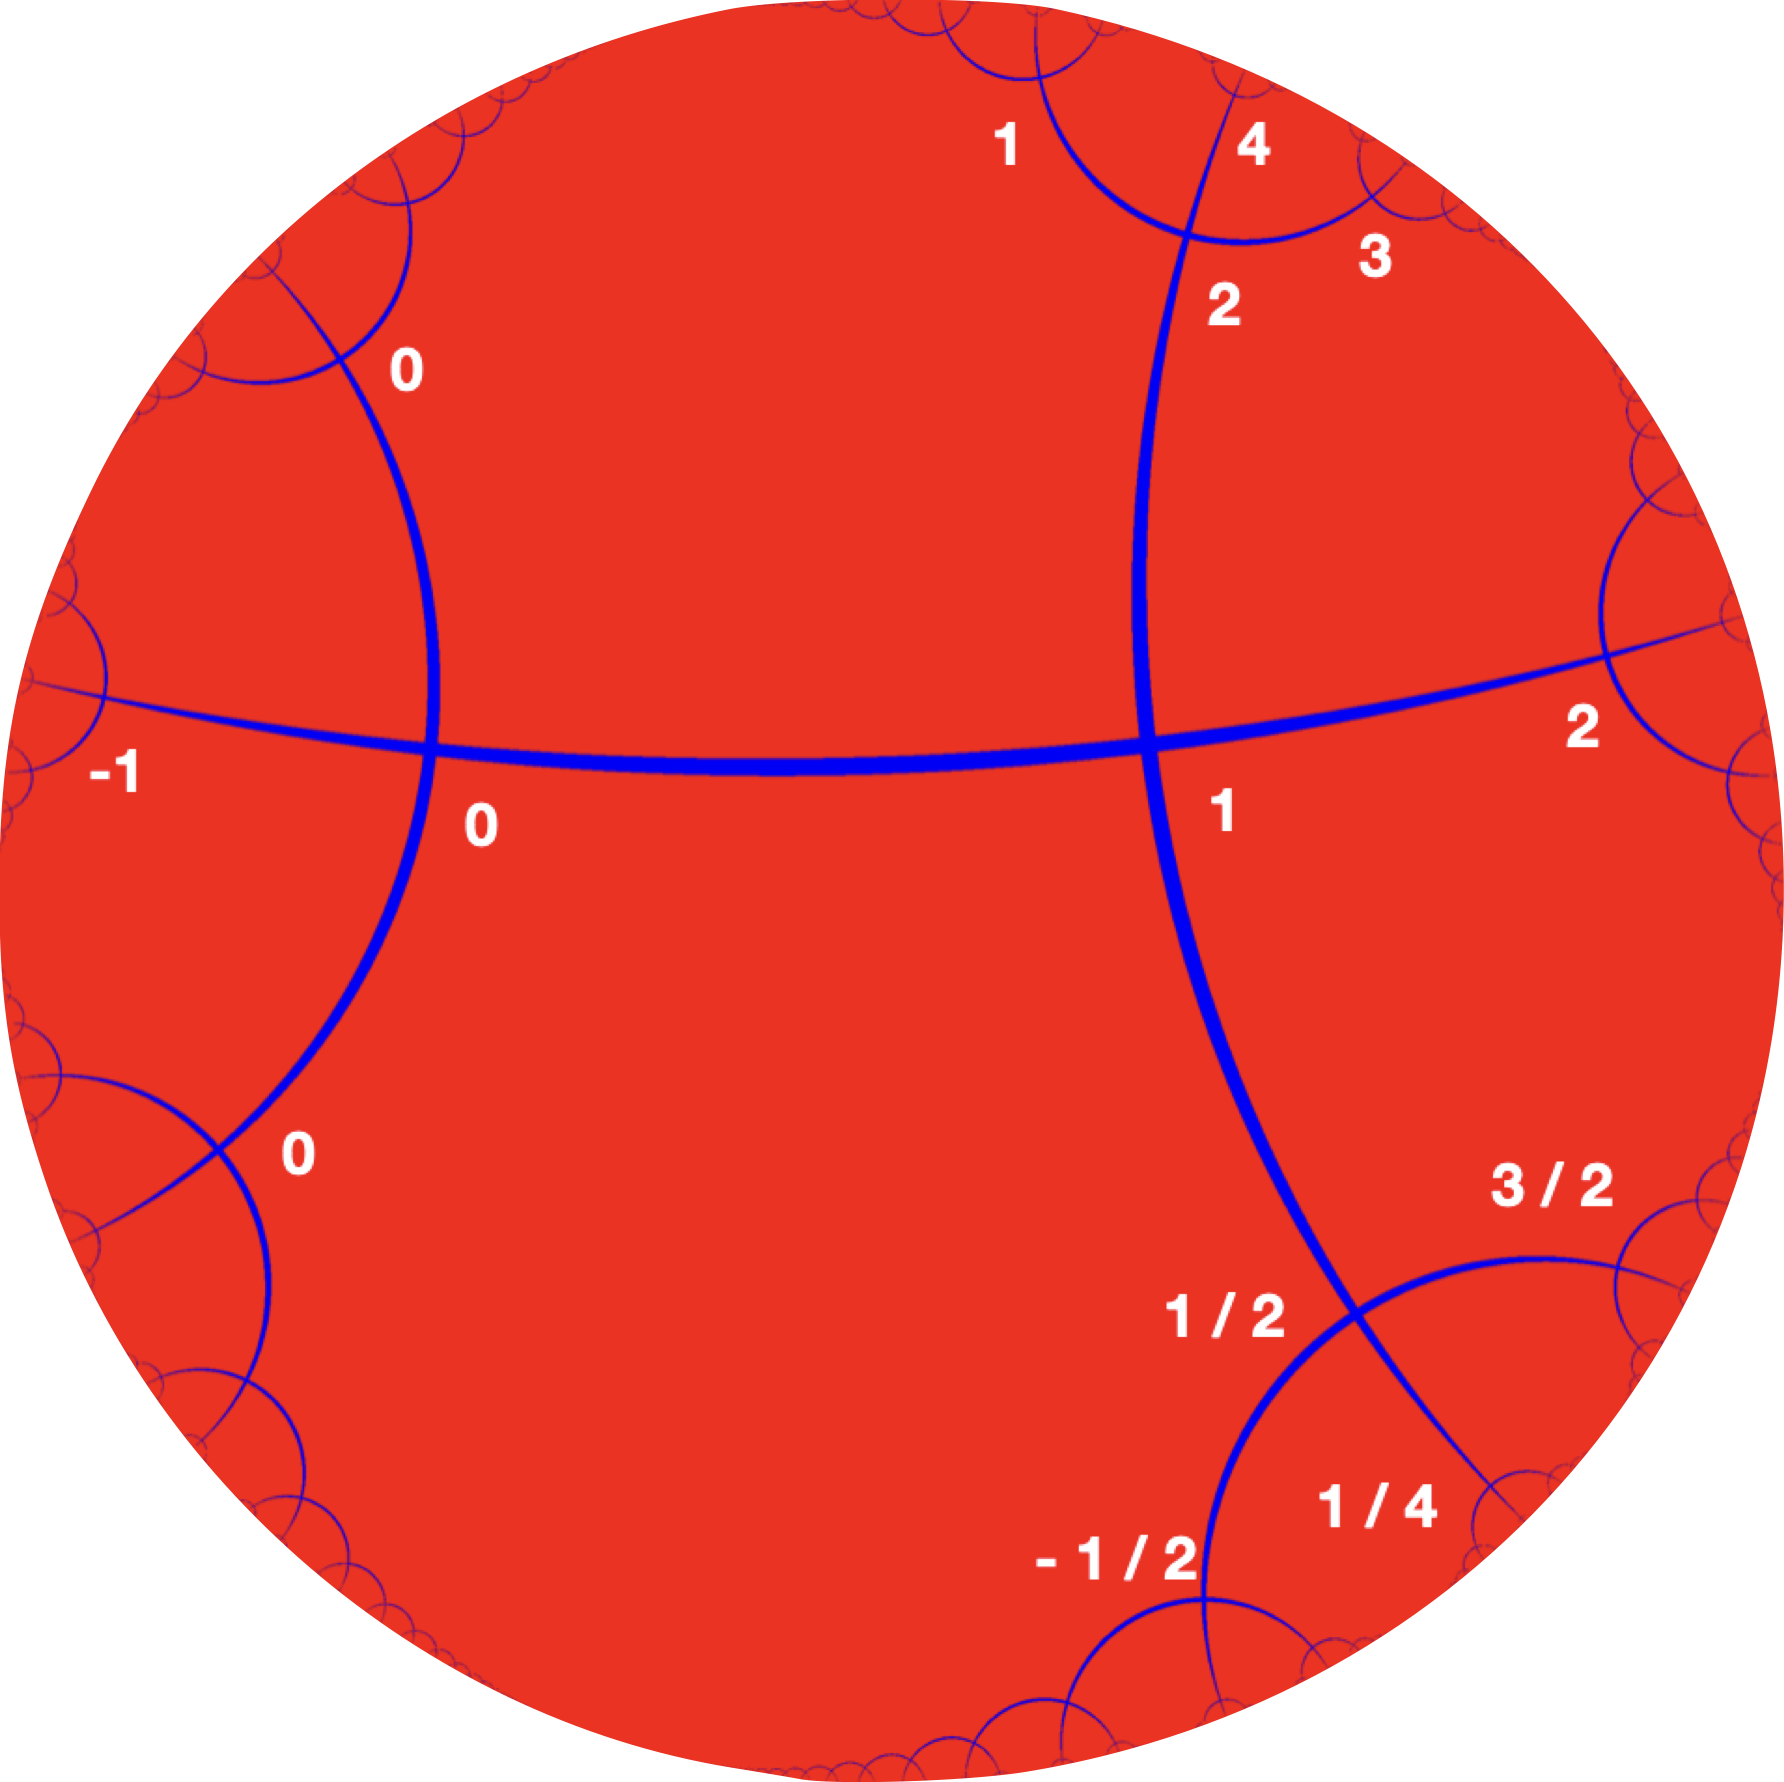
\includegraphics[width=3in]{images/assignment2.png}
\caption{管型构造上的一个切片}
\end{figure}

管型构造是在如上的离散网格基础上构造出来。如果固定加法生成元的系数为一,不断变化乘法生成元的系数,但不改变底层的网格设置,如此我们就得到一系列的切片。
然后,我们把所有的切片堆叠起来,就得到了管型构造。管型构造是异常深刻的对象。

\begin{figure}[ht]
    \centering
    \begin{tikzpicture}
        \begin{scope}[line width=0.3pt]
            \draw (0, 0) node[inner sep=0] {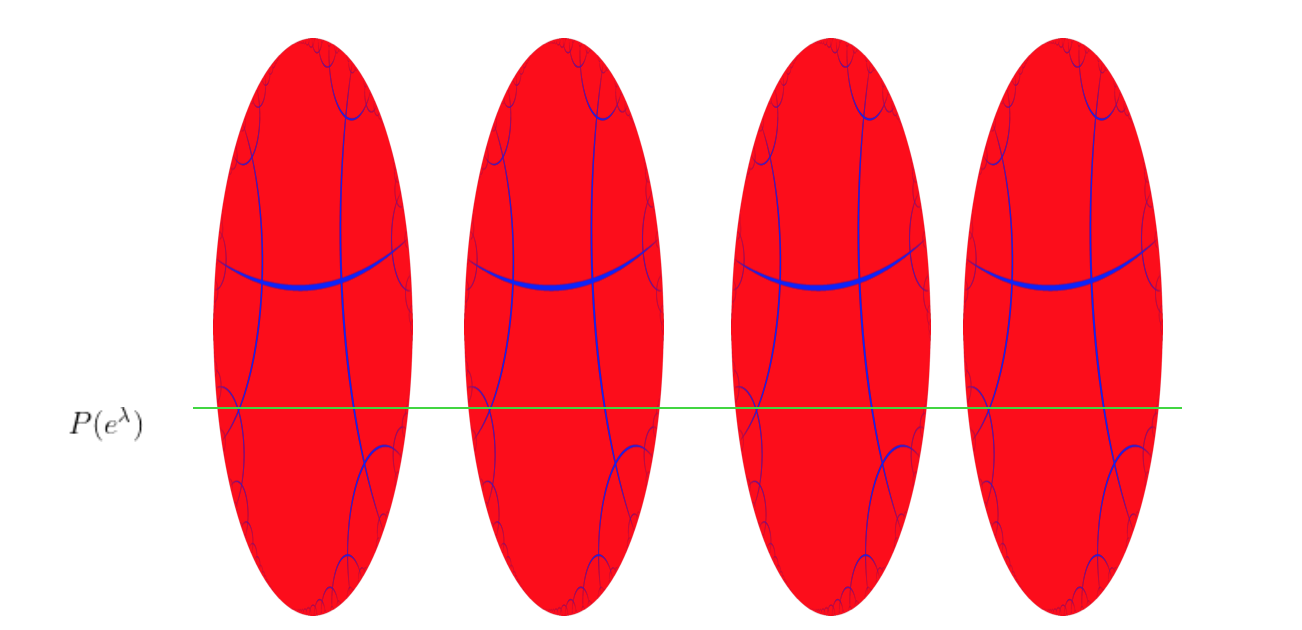
\includegraphics[width=6.284in]{images/tube.png}};
        \end{scope}
    \end{tikzpicture}
    \caption{管型构造}\label{fig:tube}
\end{figure}

加乘生成元的不同组合,会导致庞加莱圆盘上可能会有多条零线。
对乘法生成元 $e$ 来说,因为它的超越性和 Lindemann-Weierstrass 定理,只有一条零线;但对于普通的正整数,因为加乘搭配带来的整除关系,零线会有多条。
但如果我们黏合零线,我们会得到不同的 2 维流形。

同时,如果我们固定了庞加莱圆盘上的一点,每个切片都选择该位置的点,连起来就得到一条直线,我们如果研究这条直线上的赋值,
就会发现每条直线都和一个对应的多项式有关系。

这样的话,我们用一条代表多项式的线串接了无数 2 维流形上的点。如果这个构造能够成立,它会是非同寻常的数学对象。

\subsection{抽象的讨论}

让我们总结一下上面讨论的手法,并从抽象的角度来论述。

域 $F$ 上的一部分表达式构成一个群$E[F]$,完备化后得到一个几何空间$\mathbf{E}$,
于是代数的表达式群就变成了几何上的路径群$P[F]$, 同时纯代数的表达式的求值$eval$就变成了几何体上一个连续的赋值函数$A$。
在这样的设定下,我们发现几何空间上的路径可以解释为把起点映射为终点的函数;
这样就把这个几何空间上的域上的函数论同几何空间上的路径群和流联系起来,并且还可以通过赋值函数返回到域本身的问题。

这个抽象理论有过往的实例吗?有的。就是复变函数论。复变有路径积分的表达,只是在它那里,表达式只有复数域的加法。

我们可以从范畴角度来看待吗?

\newpage

\section{研究的意义}

我们认为算术表达式的几何有架通几何、分析和计算机科学的潜力。

\subsection{数学史的回顾}\footnote{参见小节\ref{subsec:newidea}里对 Benacerraf 问题的讨论。}

历史是由一系列事件构成的,一个事件触发另一个事件。人们常说亚马逊的蝴蝶煽动了翅膀,大西洋上就吹起了飓风,这一类说不清楚的事件链接,我们称之为偶然。
但是数学史的发展,源自于人们对真理的探寻,它的事件链条有认识论的意义,蕴含着某种必然性。

古巴比伦泥板上的记载显示,那时的天文学家已经知道通过累积小量来逼近星体的运动轨迹;其后,古希腊的阿基米德发展了穷竭法,汉代的刘徽发明了割圆术,
南北朝时期,祖冲之父子得出了球体积公式。古人很久之前就已经通晓利用无穷小量来解决自己的问题。这些无穷小量的技巧背后都有几何或者物理的背景。

到了 17 世纪早期,巴罗、笛卡尔、费马探索了导数的概念。1637年,笛卡尔以附录的形式发表了 La Géométrie,提出了坐标系的概念,发展了解析几何的方法,
把代数和几何结合在一起,由此才为后来牛顿与莱布尼茨的工作做了足够的准备。在 17 世纪后半叶,牛顿与莱布尼茨建立了微积分的框架。

在 17、18 世纪,无穷小量的基础还不牢靠,引发了大量的讨论。微积分经由欧拉等人的工作,逐步变成了现代的形态。实分析的严密理论到了19世纪经威尔斯特拉斯、
戴德金等人的工作,才逐渐完备起来。更由此引出了对集合、自然数、实数和数学基础的研究。

欧几里得第五公设有上千年的讨论,高斯、罗巴切夫斯基和鲍耶开创了非欧几何的研究。由此引发的问题,让几何也成为了数学基础研究的一部分。

希尔伯特把几何学归结为算术,并提出了形式主义的纲领,但被哥德尔否定。在对希尔伯特的第十个问题的研究中,人们需要算法的严密概念,导致了 1930 年代计算机科学的建立。

我们的一个疑问:从分析学和几何学研究里一步步诞生出来计算机科学,但为什么计算机科学本身,从方法的内核上讲,却远离分析学和几何学呢?
这从数学的角度讲是对的吗?

\subsection{分析部分}

从附录的章节,我们很容易看到,算术表达式空间上的一条的路径其实对应了一种特别的积分。传统的微积分,刻画一个变化过程,用的是累加小量的思想;
也可以用累乘方法,去刻画复利的累积、放射性的衰减,只需要用对数来帮忙,把累乘转换为累加,所以累乘和累加是同一套理论;
但如果我们用加乘混合的方式来刻画一个过程,背后对应的是什么理论呢?

当然,我们可以有拓扑群上抽象的积分,从这个角度讲,我们的处理手法可以归为此种情况。但算术表达式视为拓扑群的观点,在我所知的范围,并没有见诸文献。
因为大家都在讨论数,而非表达式,更遑论表达式的几何。抽象地看算术表达式的几何也是 $SL(2)$,但和以往 $SL(2)$ 理论不一样的是,它的实现是不同的,
这有两个后果:(一)把 $SL(2)$ 抽象理论用一种不同以往的方式引入到了算术表达式理论或者数论里;(二)提供了潜在的新工具去解决 $SL(2)$ 抽象理论里的问题。
\footnote{对尤亦庄老师的问题——如果这套理论可以发展出来,它和现在的 SL(2) 的理论有何不同?这里给出了第一个回答的思路}
当然,也会有个问题:不同的实现或者表示之间除了便利性有差别,它们之间有无本质上的区别?

从以上分析,我们可以看到算术表达式的几何同分析学有天然的联系。如果说分析学是无穷小算术的代数理论,算术表达式的几何意味着什么呢?这需要我们重新思考函数的概念。

我们给定了实数域$R$上的函数$k$,于是我们可以引入算术表达式空间$H$上的映射$l$,使得下图可交换。

\begin{center}
    \begin{tikzcd}
        H && H \\
        R && R
        \arrow["l", from=1-1, to=1-3]
        \arrow["\nu"', from=1-1, to=2-1]
        \arrow["\nu", from=1-3, to=2-3]
        \arrow["k"', from=2-1, to=2-3]
    \end{tikzcd}
\end{center}

其中的$\nu$是表达式的估值函数。此时,称我们把函数$k$提升为映射$l$,或者映射$l$的投影是函数$k$。

抛去符号的外衣,上面的交换图在说明我们可以用几何流来表达函数的效果,而几何流本身就是函数的计算过程或者说一种特别的微积分学。
沿着加线的计算过程,就是普通教科书上的积分过程;沿着乘线的计算过程,对应纯乘法的积分过程。所以,算术表达式空间$H$可以理解成一个微积分的理论空间。
\footnote{关于效果和过程的具体内容,见 \ref{sec:learnandhalt} 节的讨论}

我们知道一个演化过程有它内在的对称性,有趣的是这个对称性能否在算术表达式空间$H$有所体现吗?会存在一条特殊的路径代表着一种特殊的微积分计算过程,
它可以分析一些非线性函数?这个思路能否打开对一大类非线性函数的研究?能否把群论和函数论联系起来?
\footnote{对尤亦庄老师的问题——如果这套理论可以发展出来,它和现在的 SL(2) 的理论有何不同?这里给出了第二个回答的思路。}

\subsection{几何部分}

如果能严格论证清楚管型构造的存在,它必定是一个极端重要的几何对象。

我们认为算术表达式的几何应该也能为几何研究本身开辟新的计算途径。
比如,交换子是否可以用来计算曲率呢?\footnote{受教于蒋文峰老师的指导}
对某些适用的流形,零线是否有助于计算基本域?能否用来做单值化呢?
这些都是可以看到的可能性。

\subsection{计算部分}

通过邱奇编码(Church encoding),我们直接可以把算术表达式空间变成程序的几何空间。\footnote{感谢李熙老师的指导}

计算不只有算术和代数的方式,也可以通过几何来计算:考察发散级数

为机器学习提供新的表达手段和优化途径。

刻画计算过程,让我们可以讨论不停机的计算过程。\footnote{参见小节\ref{sec:learnandhalt}}

\newpage

\section{更多的思考}

\subsection{学习与停机问题}\label{sec:learnandhalt}

在附件二的译后记中,我提及一篇少为人知的重要论文

\begin{displayquote}
1996 年 R. Lathrop 在 ICML 上发表了 On the Learnability of the Uncomputable ,
论文表明通过分析程序运行的时空行为,在概率意义上停机问题可学习。论文在可计算性和可学习性之间给我们找到了一块落脚石,
同时论文的分析方法和算法信息论(AIT)里 Chaitin 常数 $\Omega$ 的渐进可计算性似乎有更进一步的联系。
\end{displayquote}

在附件一中,我有这样几段话,我把它们列在一起,来表明我的一种一致的观点

\begin{displayquote}
在工程实践中,我们有两种方式使用一个计算机程序。一种是使用它的最终效果,一种是使用它的计算过程。
前者的例子是程序库的各种标准例程,比如 $\sin$、$\cos$ 等等,我们不在乎它的实现细节和计算的中间状态,只在乎最终结果。
后者的例子是打游戏,游戏程序循环的每一步,都导致我们用户在音视频上的某种体验,整个计算过程都是我们需要的。
\end{displayquote}

但在可计算性的理论里,我们仅仅考虑的是能够停机的偏函数,为什么我们不能考察整个计算过程呢?
我的理解是,我们缺乏一种数学语言,去刻画一个计算过程。这种数学语言的缺失,很早很早之前就埋在了数学的发展中。

\begin{displayquote}
人们常说,数和形是数学的基本主题。让我们看一下数的早期历史。
从石器时代非洲的骨刻,我们可以看到数的概念表征和计算过程是浑然一体的,这种表征非常繁琐,计算的能力也非常有限。
其后,数的表征,经过古埃及的不成熟形态,到达了古巴比伦的数位制。

在这个历史过程里,人们遗忘了一个隐藏的巨大世界—那就是表达式,或者说计算过程。
数作为一种表征,本来就是计算过程的高度凝练的表达,但它一旦符号化后,就成为我们追求的目标。
于是,我们往往关注计算过程的结果,而忽视了过程本身蕴含的众多信息。

过程比结果更重要。
\end{displayquote}

算术表达式的几何提供了一种可能,在这里计算过程可以被实现为一个几何上的流。

\subsection{机器能否数数的思考}

2021 年 1 月集智年会上我做了一个小的分享,去探讨机器能不能数数的问题。

表面上看似乎不是问题,机器本来不就是高级版本的计算器嘛!实则不然,我其实在这里提了
一个不同于图灵测试的智能体的创造性测试问题。图灵测试是以人类智能为标准的,而这里的
机器数数的测试问题则是以一种超出了人类智能的方式来设问的。

在演示文档中,我有一层层的剥开这个问题,先考察生物和认知里的数,继而从目前人类的形
式定义去考察,发现想把这个问题定义清楚都比较困难。 困难在于,无法简单的排除掉智能体
可以创造出和人类不同的数的形式,但这种情况下,你无法给出一个数的标准定义,从而也很
难给出能不能数数问题的测试标准。 最后一段,我尝试用强化学习的思路,创造一个生存环境,
智能体必须通过计数的方法来获得更优的选择,然后不限定智能体的策略的制定,如此从侧面
去考察数的创造。

这种强化学习的思路,最终还是通过报酬或者激励的量化来驱动策略的搜索,也就是把数的创造
问题化归为一个势能面上的寻优。这背后是一种\textbf{几何式的元数学}观点。

扩展开来,这里面其实有个很深的智能体之间彼此理解的问题。
我对沙漠蚁计步的能力就很好奇:沙漠蚁在觅食时可以走很复杂的路线,但是它们一旦归巢,
就会直奔巢穴的位置。 沙漠蚁在这里展现出来的空间路径积分的能力,其实不比人类最开始掰
手指头数那么几百个数要低。我想的是数学能力其实是一种具身性的能力,而数学形式也受具
身性的影响。 想要隔着物种或者其他的隔阂去理解的话,必须得深入到那个具身环境里去理
解。但我倒不是否定柏拉图理念式的数学,我是想探索这些不同具身环境下的数学形态的某种
公约数。当生物逐渐从昆虫演化到了哺乳动物,它们在海马体里出现了导航神经细胞,这些细
胞有六边形的活跃模式。那么这种神经层面上六边形活跃模式对应的几何, 怎么和我们心理
层面的几何挂上钩的呢?从数学角度如何理解呢?所以还可以跨越神经、认知和数学,去思考
更多。

上面提到的公约数可能也是理解人类符号化知识的一个有趣切入的方向。考察这种异与同背后,
其实还有一个问题是什么是真实?有没有这种真实? 如果没有这种真实,智能体之间能互相理
解吗?这背后的指涉,远不止在具身性数学的探讨,如今混乱的人类世界或许也需要深刻反思
这个问题。

\subsection{环形的推理结构}

因为上面提到了多种数学形态,和寻求公约数。我在想另外一种推理的方式。我们学习实数理论
或者复变函数时,不少教科书就采用了一种环式的论证,它不是循环论证,而是通过一个环形的
蕴含来论证一定条件下的概念间的等价性的。

我在想,这种环式的推理是可以被挖掘的,有趣的一个问题,这个环包围的空有没有意义呢?
你可以想到同伦或者某种语义的空间。它就不单纯是推理的链条了。相反,我们要跳出推理链条,
从链条的外面来看。

有趣的是,在算术表达式的几何里,我们就是从词向量这种语义空间的构造开始的。而得到的算术
表达式空间,可以被赋值函数的等值线与梯度分解。我们知道等值线就是逻辑上的等值关系,
梯度可以理解成一种特殊的推理机制。既然算术表达式被几何化了,那么是否有可能一个命题体系
也可以被几何化?

更进一步,希尔伯特把几何算术化,所以我们能把希尔伯特的思路反过来吗?给出一个几何式的元数学?

\subsection{新的观念}\label{subsec:newidea}

寻找新的思想和方向是我们这一代人的任务,努力向下去思考。我们不能仅停留在算术表达式的几何上,
我们需要提炼出新的数学结构和新的数学观念。

虽然还言之尚早,但算术表达式的几何或许会把我们引向一种“过程与形式”的数学。
区别于“形与数”的数学中两个要素是彼此割裂的,在“过程与形式”的数学中,两个要素是对偶统一的。
只要能在“过程与形式”的数学中,恰当的引入“真”,这个体系就可以先于“数”与“逻辑”存在,
我们可以从“过程与形式”里衍生出来“数”与“逻辑”。

\begin{figure}[ht]
\centering
\begin{tikzpicture}
\draw (6, 2) node[inner sep=0] {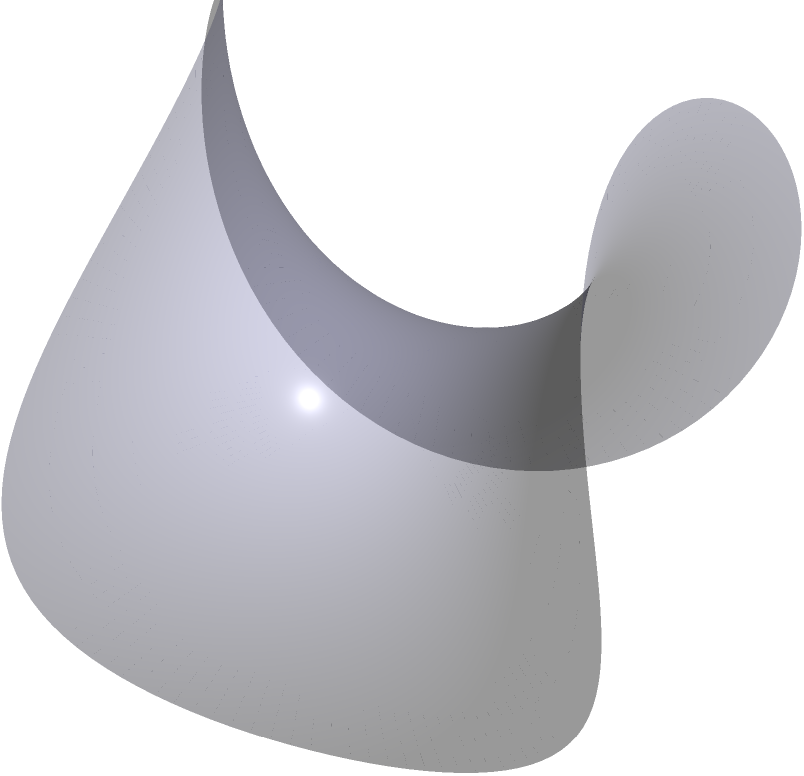
\includegraphics[width=4in]{images/ennepers.png}};
\node [anchor=225, black] at (9,6) {几何};
\node [anchor=225, black] at (9,-3) {分析};
\node [anchor=225, black] at (2,6) {计算};
\node [anchor=225, black] at (0,0) {学习};
\node [anchor=225, black] at (6,2) {算术表达式几何};
\end{tikzpicture}
\caption{知识的极小曲面}
\end{figure}

康德有论述“先天综合判断”,几何作为命题都呈现为“综合命题”,肥皂泡的几何式知识观有可能会暗合康德的理论。
这个知识观可以形式化为上面说的“过程与形式”的数学,而算术表达式几何就是这个“过程与形式”的数学的第一个例子。

如果要讨论怎么恰当的引入“真”,必须参考两个问题:Benacerraf-Field 挑战和 Wigner 的数学有效性问题。

Benacerraf-Field 挑战首先由 P. Benacerraf 提出,后由

\end{document}






